\section{Introduction}\label{sec:intro}
The discovery of the standard model (SM) Higgs boson at the LHC~\cite{ATLAShiggs,CMShiggs} 
presents a unique opportunity to search for physics beyond the SM (BSM) using the Higgs boson as a search
tool. Given the small value of the Higgs production cross section in the standard model, 
any BSM scenario predicting new mechanisms for Higgs boson production can be investigated 
with dedicated searches, using the known Higgs mass to suppress SM background processes.


This Chapter presents a search of this kind in pp collisions at 13 TeV using data from the CMS detector at the CERN LHC.
Events with two photons consistent with a Higgs candidate are selected and categorized
according to the $p_{T}$ of the Higgs candidate, the presence of additional 
Higgs to $b\bar{b}$ or Z to $b\bar{b}$ candidates, and the estimated resolution of the diphoton
pair. Motivated by supersymmetric (SUSY) scenarios, we use the razor variables~\cite{razor2010, rogan}
\MR and \Rtwo  -- extensively dicussed and illustrated in
Chapter~\ref{chapter:razor} -- to define search regions that may contain additional events above the SM prediction
if a BSM Higgs production mechanism is present.  
The contribution in the search regions from the non-resonant QCD background is distinguished from a potential BSM 
Higgs signal using the shape of the diphoton mass distribution. The search uses $2.3$~$\mathrm{fb}^{-1}$ of 
integrated luminosity collected in 2015 and $12.9$~$\mathrm{fb}^{-1}$ collected in 2016. 


In Run 1 of the LHC, a similar CMS analysis~\cite{SUS-14-017} reported an excess of $H \to \gamma \gamma$ 
events with $\mathrm{M_R}\approx 400$~\GeV and $\mathrm{R^2}>0.05$ with a local (global) significance of
$2.9\sigma$ ($1.6\sigma$). Motivated by the Run I result, we consider a
SUSY simplified model in which bottom squarks are pair produced and decay
to a bottom quark and the next-to-lightest supersymmetric particle (NLSP), 
$\tilde{\chi}^{0}_{2}$, with $100\%$ branching ratio.
The NLSP subsequently decays to a Higgs boson and the lightest 
supersymmetric particle (LSP), $\tilde{\chi}^{0}_{1}$, with $100\%$ branching ratio. 
We assume that the mass difference between the NLSP and the LSP is $130$~GeV,
just above the Higgs boson mass.
The relevant decay topology in the simplified model is shown in Figure~\ref{fig:T2bH}. 
The cross section for this simplified model is assumed to be the same
as the standard sbottom pair production cross section~\cite{Borschensky:2014cia}.
Such a signal model is observed to produce event kinematics consistent with the
excess observed in Run I data and is not ruled out by searches in
other final states and decay channels. This search is interpreted using
the sbottom pair production model as the benchmark, and we derive limits 
on the production cross section as a function of the sbottom mass and the
LSP mass.


\begin{figure}[ht!]
\centering
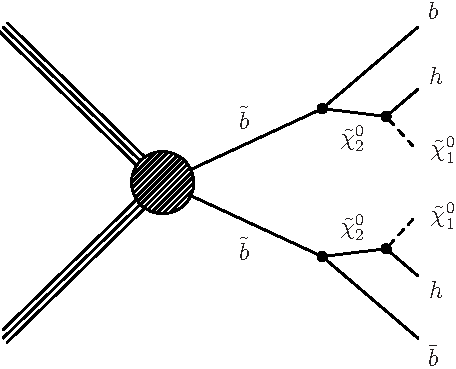
\includegraphics[width=0.4\textwidth,angle=0.]{figs/T2bH.pdf}\\
\caption{Diagram illustrating the SUSY benchmark simplified model of bottom squark decays to a Higgs boson, a b-jet, and the LSP.
       \label{fig:T2bH}}
\end{figure}

\section{Summary of the 8 TeV Results}\label{hgg:8TeVsummary}
The first version of the analysis to be presented in this Chapter was
carried out by CMS~\cite{SUS-14-017} and studied in more detailed in
Alex Mott's thesis~\cite{AMott}. Here, a summary of the main
results is given as is relevant for the discussions to follow.

The 8\TeV analysis selects events in a very similar fashion to the one
presented in this Chapter. It categorizes events based on the Higg
candidate $p_{\mathrm{T}}$, the photons energy resolution, and the
invariant masses of ther possible b-jet pairs -- indeed, intended to
target an extra Higgs or Z boson on the event. The final results yield
that most of the search bins were consisten with the SM expectations,
and the results were interpreted as cross section limits on the
neutralino/chargino production in the context of SUSY simplified
models. The observed significances for all the search bins are shown
in Figure~\ref{hgg:significance8TeV}, while the limit on the
neutralino/chargino production as a function of the chargino mass is
shown in Figure~\ref{hgg:limit8TeV}. Although, most of the search bins
were consitent with the SM expectations, an interesting excess of
events was observed in the most extreme bin -- that with the highest
\MR and \Rtwo boundaries -- in the High-Resolution (HighRes) event
category, see Figures~\ref{hgg:table8TeV} and~\ref{hgg:highresRazor8TeV}, where both photons forming
the Higgs cadidate are require to have an energy resolution better
than 1.5\%. This excess corresponds to a 2.9$\sigma$ (1.6$\sigma$)
local (global) significance. Such an excess, despite the limited
number of events, is interesting for mainly two reasons: first, it is located at relative
high values of \MR ($\sim 400$\GeV) and low values of \Rtwo (below
0.05), see ~\ref{hgg:highresRazor8TeV} for more detail, and therefore
suggest a characteristic mass scale and that they contain relative low
$\ETm$ values. second, that the diphoton invariant mass is
consistent with that of the SM Higss boson and therefore any possible
model to explain such an excess should at least contain a one SM Higgs
boson. The diphoton invariant mass for the events that lie in the bin
with the excess are shown in~\ref{hgg:mgg8TeV}. The search presented
in this Chapter is largely inspired on it 8\TeV counterpart, but with
significant differences when it comes to the backgrouns estimation
techniques. In addition, the proposed simplified model shown
in Figure~\ref{fig:T2bH} -- which is studied in great detail in
Chapter~\ref{hggPheno} -- shows some consitency with the excess
observed in the 8\TeV CMS result.
\begin{figure}[ht!]
\centering
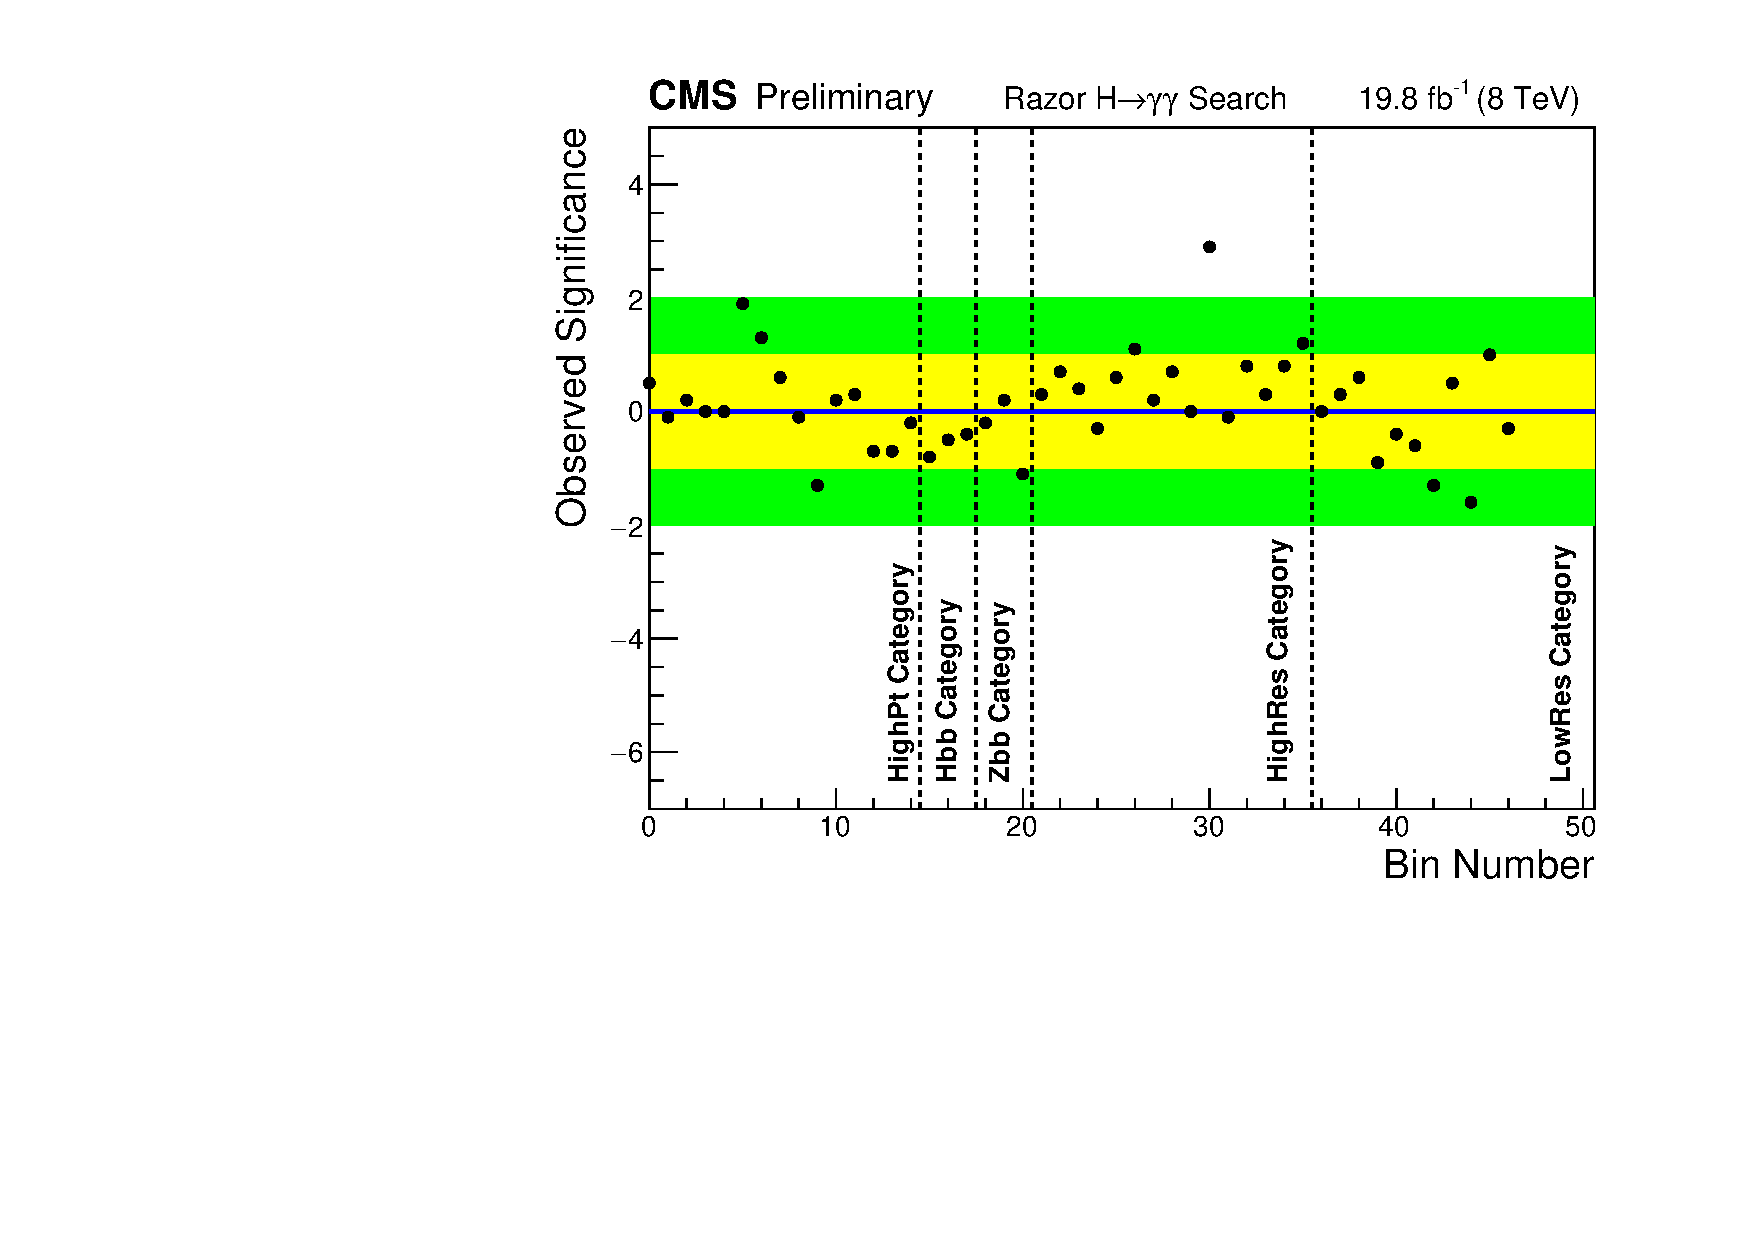
\includegraphics[width=0.6\textwidth,angle=0.]{hgg/SignificanceVsBin_8TeV.pdf}\\
\caption{Summary of the  results in the HighRes category for the 8\TeV
  version of the analysis.
       \label{hgg:significance8TeV}}
\end{figure}
\begin{figure}[ht!]
\centering
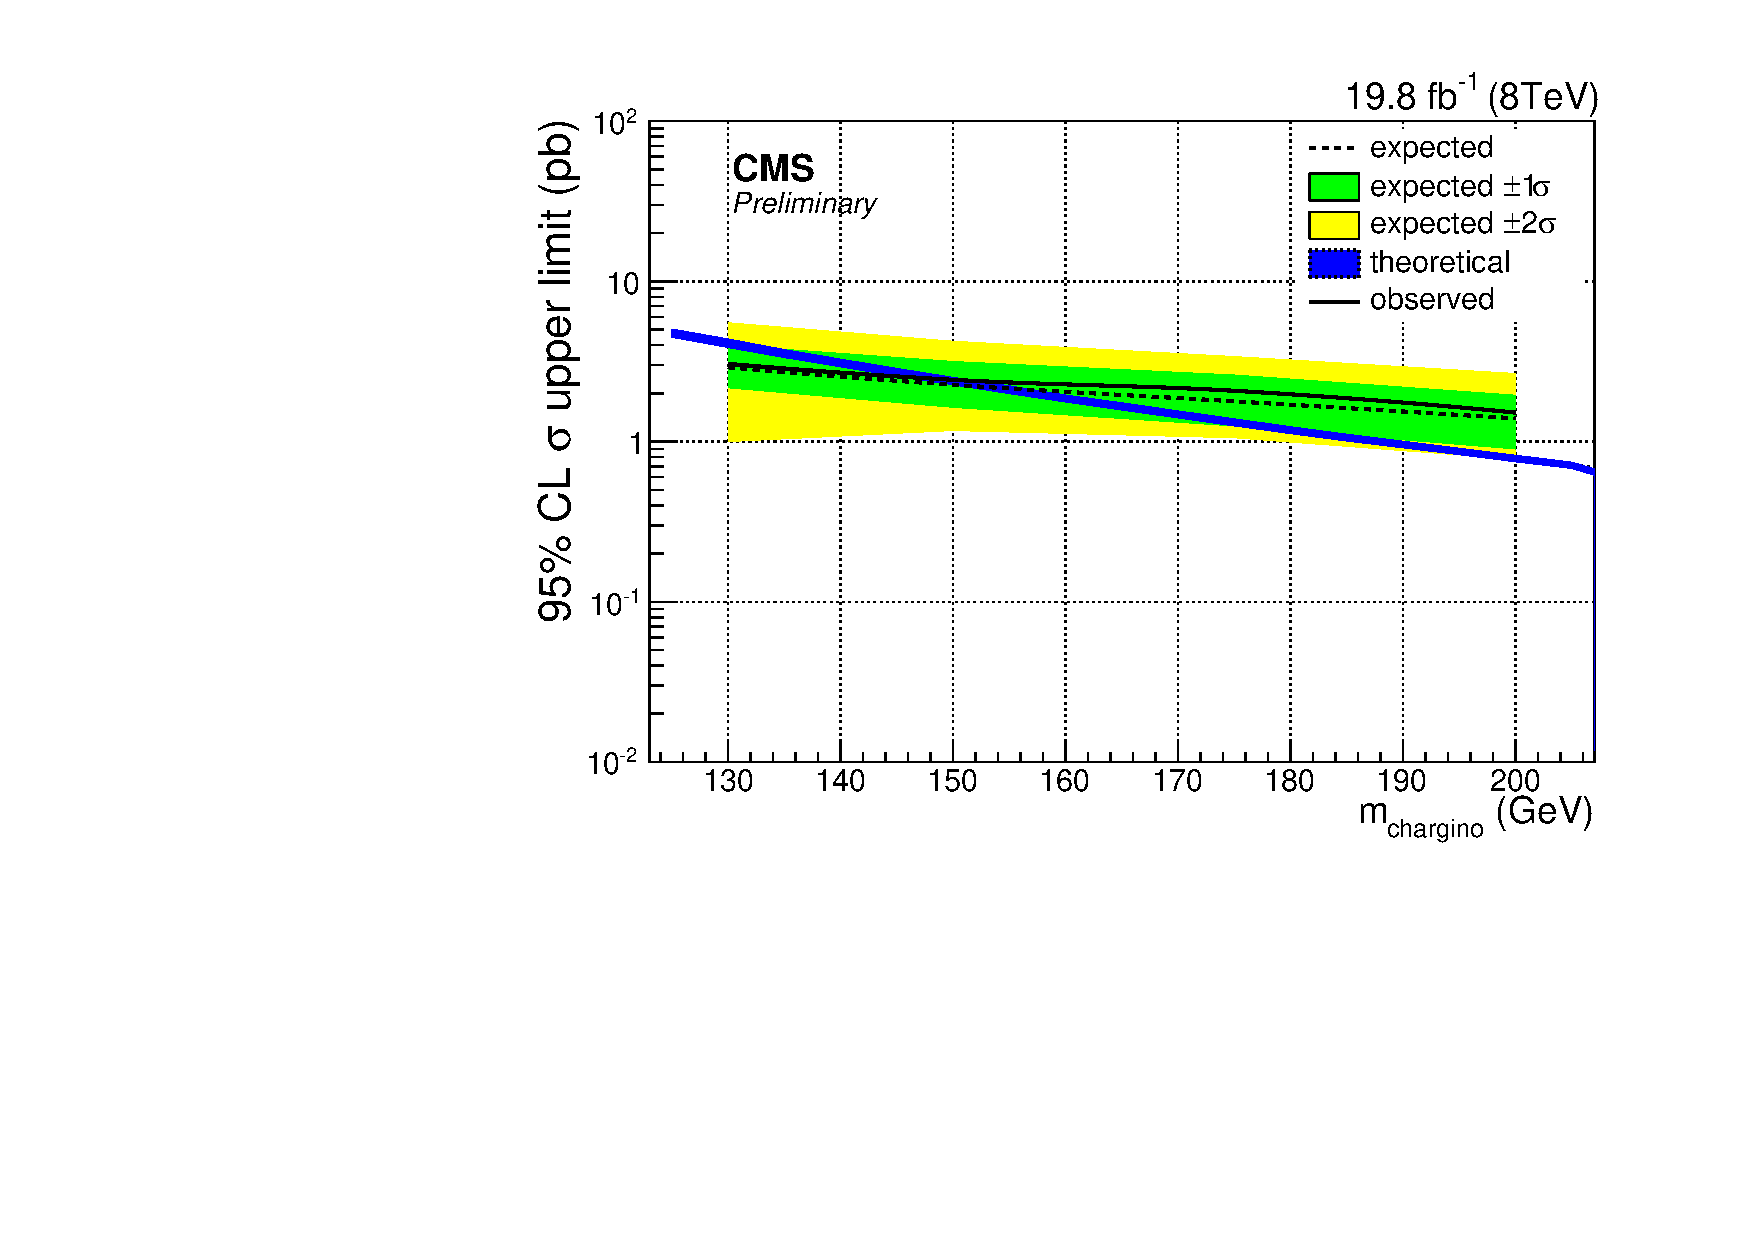
\includegraphics[width=0.6\textwidth,angle=0.]{hgg/expected_exclusion_WH_1D_OBS.pdf}\\
\caption{Summary of the  results in the HighRes category for the 8\TeV
  version of the analysis.
       \label{hgg:limit8TeV}}
\end{figure}
\begin{figure}[ht!]
\centering
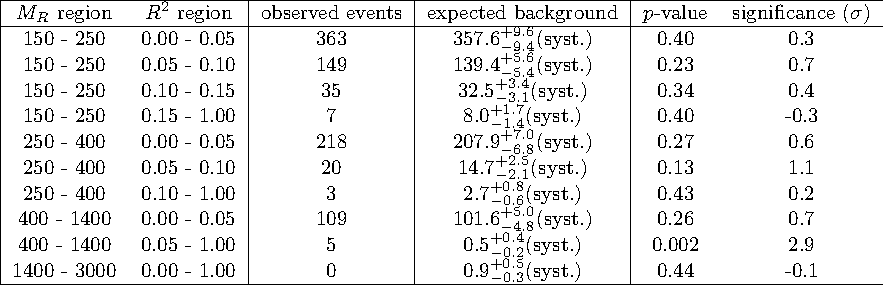
\includegraphics[width=0.6\textwidth,angle=0.]{hgg/Table9.pdf}\\
\caption{Summary of the  results in the HighRes category for the 8\TeV
  version of the analysis.
       \label{hgg:table8TeV}}
\end{figure}
\begin{figure}[ht!]
\centering
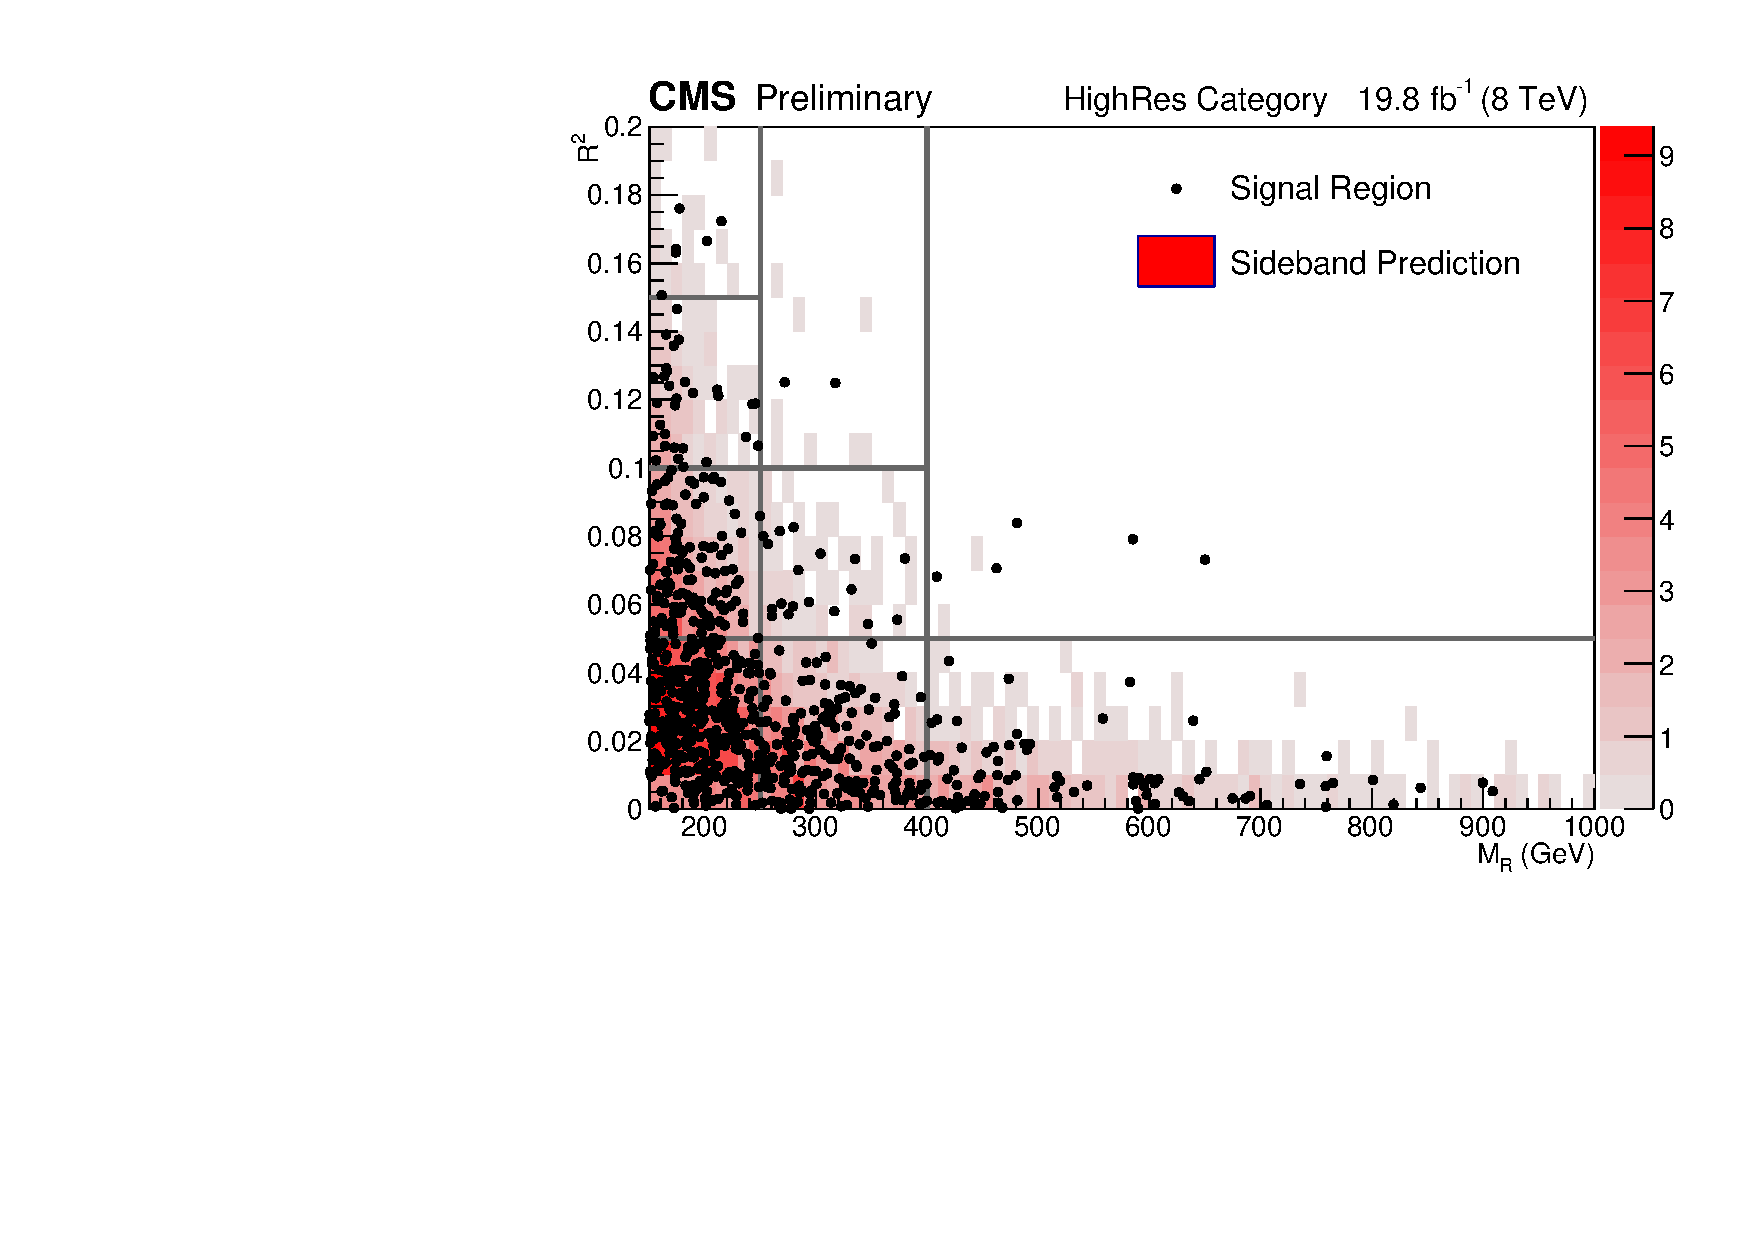
\includegraphics[width=0.6\textwidth,angle=0.]{hgg/HggRazor_MRRsq_highres_8TeV.pdf}\\
\caption{Summary of the  results in the HighRes category for the 8\TeV
  version of the analysis.
       \label{hgg:highresRazor8TeV}}
\end{figure}
\begin{figure}[ht!]
\centering
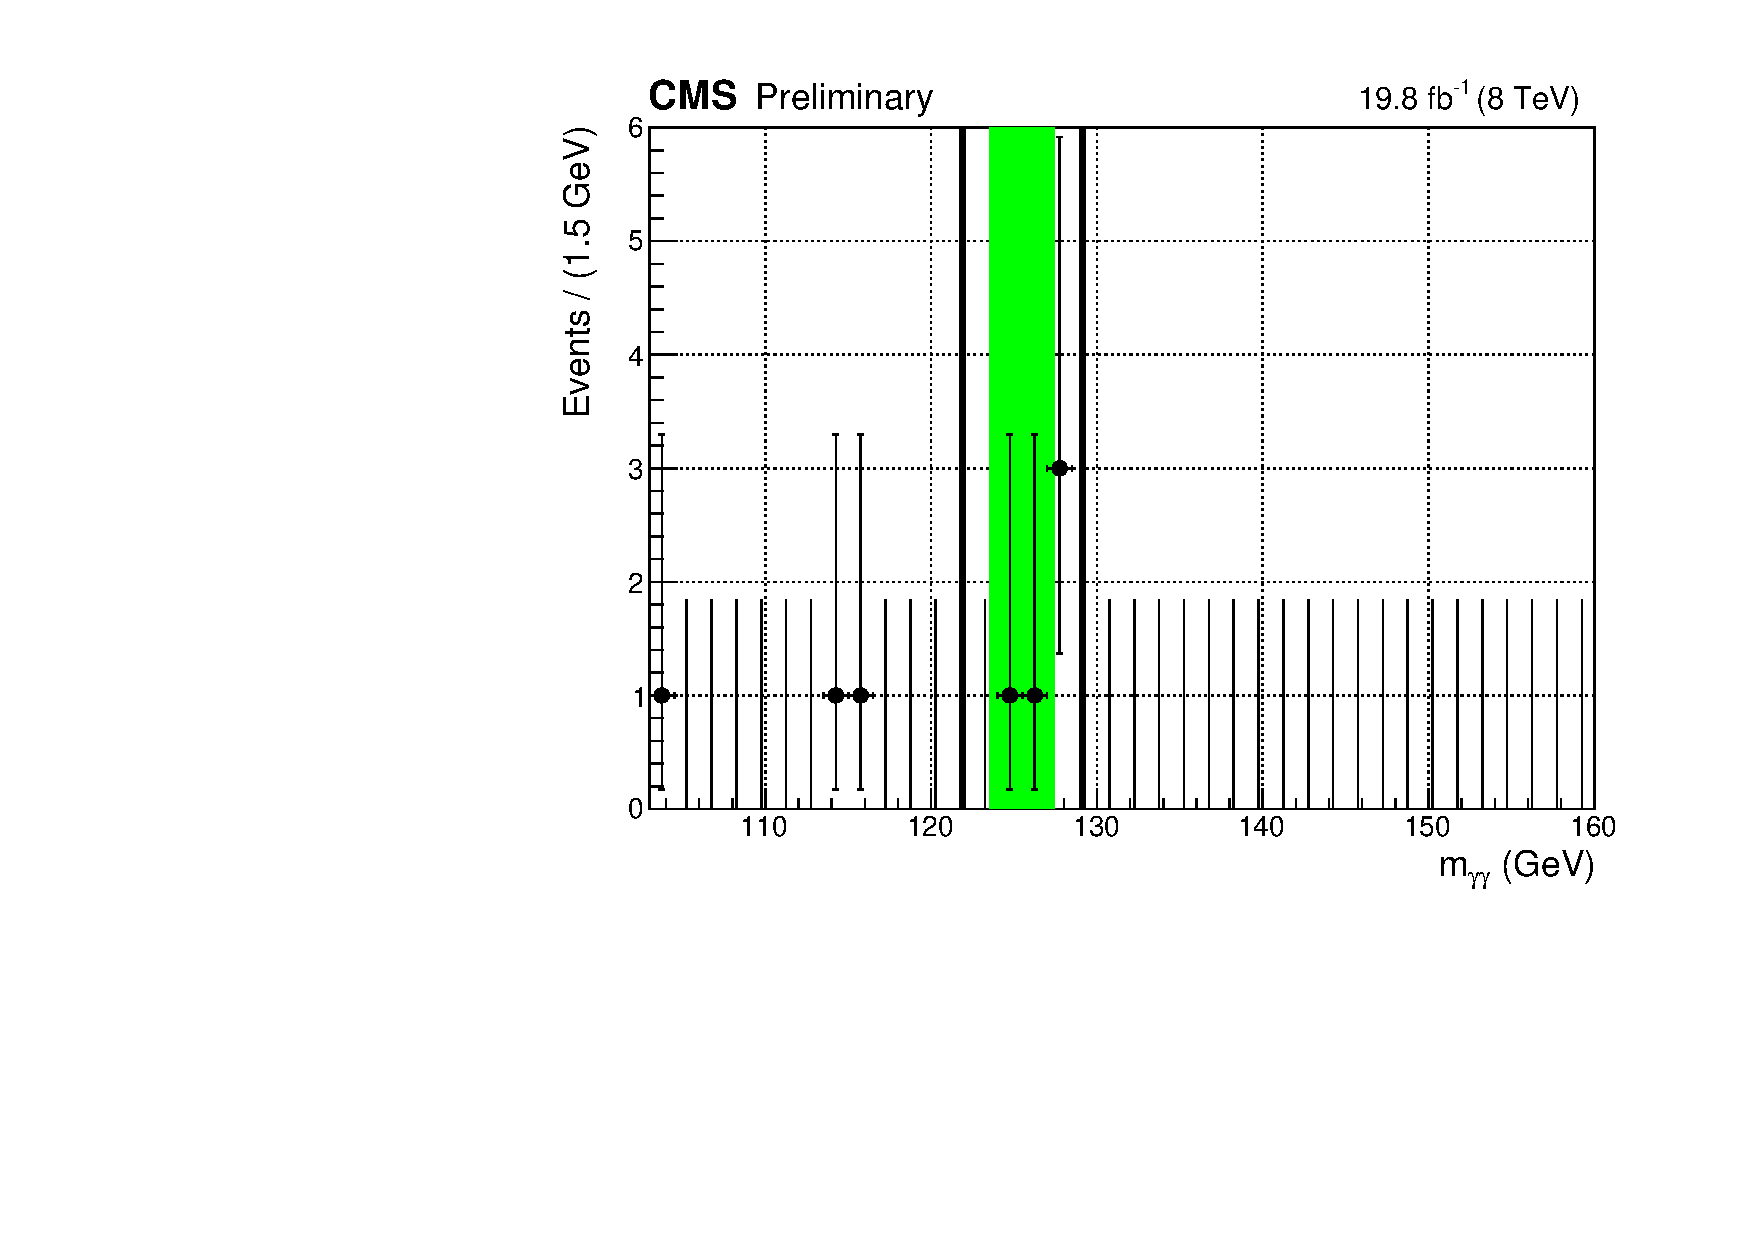
\includegraphics[width=0.6\textwidth,angle=0.]{hgg/HggMassPlot_HighRes_8TeV.pdf}\\
\caption{Summary of the  results in the HighRes category for the 8\TeV
  version of the analysis.
       \label{hgg:mgg8TeV}}
\end{figure}
\section{Object Selection}\label{sec:ObjectSelection}


Photon candidates with $p_{T}>25$~\GeV falling in the barrel region ($|\eta|<1.4442$) are selected if 
they satisfy identification requirements based on the shower shape in the electromagnetic calorimeter, the hadronic to
electromagnetic energy ratio, and the isolation in a cone around the photon direction~\cite{Khachatryan:2014ira}. 
To satisfy the isolation requirement, the sum of the energies of PF candidates near the photon must be 
smaller than a specified cut value.  Isolation cuts are placed separately on energy from charged hadrons, 
neutral hadrons, and photons.  Each isolation sum is corrected for the effect of pileup by subtracting the
average energy deposited into the isolation cone estimated using a random
sampling of energy density in the event. Photon objects are rejected if 
they match an electron candidate. The photon identification requirements correspond to a loose working 
point with an efficiency of about $90\%$.


The measured energies of the photons are corrected for clustering and local
geometric effects using an energy regression trained on
 Monte Carlo simulation~\cite{Khachatryan:2015iwa}. This regression gives a significant
improvement to the energy resolution of the photons and provides an estimate of the uncertainty of the energy measurement. 
This uncertainty estimate is used in this analysis to categorize events into high and low resolution categories. 


Jets are reconstructed using a global event description based on the CMS 
particle flow (PF) algorithm~\cite{PF1,PF2}. Individual particles (PF candidates) are reconstructed 
by combining the information from the inner tracker, the calorimeters, and the muon system. 
Charged PF candidates associated to a vertex other than the primary one are considered pileup and are rejected.  
The remaining particles are clustered into jets, using the \textsc{FastJet}~\cite{fastjet} implementation 
of the anti-\kt~\cite{antikt} algorithm with the distance parameter $R=0.4$. Jets are required not to 
overlap with either of the two photons; this requirement is imposed by the condition $\Delta R = \sqrt{(\Delta \eta)^2 + (\Delta \phi)^2}>0.5$. 
The vector sum of the reconstructed $\pt$ of the PF particles is used to quantify 
the missing transverse momentum $\ptvecmiss$ in the event.  Events with detector- and beam-related noise that can mimic 
event topologies with high energy and large $\ETm = \left|\ptvecmiss\right|$ are filtered using dedicated 
noise reduction algorithms~\cite{Chatrchyan:2011tn,Chatrchyan:2012lia,Khachatryan:2014gga}.


The combined secondary vertex (CSV) tagging algorithm~\cite{btag8TeV} is used to identify 
jets originating from the showering and hadronization of b quarks. A loose working point is used
which yields a mistag rate that is approximately $10\%$.
Jet pairs are identified as $\bbbar$ candidates if the two jets satisfy the CSV requirement. 
Among all $\bbbar$ candidates in the event (if there are any), the pair with mass closest to 125~\GeV (91.2~\GeV)
is chosen as a $H \to \bbbar$ ($Z \to \bbbar$) candidate. Events are not required to contain a 
$\bbbar$ pair; the presence or absence of a $H \to \bbbar$ or $Z \to \bbbar$ candidate with mass in the 
specified range is used in the event classification procedure described in Section~\ref{sec:EventSelection}.


\section{Event Selection and Analysis Strategy}\label{sec:EventSelection}


We select events with two photons that satisfy the identification criteria described
above. If multiple photon pairs are identified, the pair with the largest scalar sum of the 
transverse momenta of the photons is chosen as the Higgs candidate. 
The Higgs candidate must additionally have leading photon $p_{T}$ greater than $40$\GeV, 
and diphoton mass between $103$\GeV and $160$\GeV. 


In addition to the diphoton Higgs candidate, we require at least one additional jet
with $p_{T}>30$\GeV and $|\eta|<3.0$. The Higgs candidate and all identified jets
are clustered into hemispheres according to the Razor~\textit{megajet} algorithm\cite{razorPRD}, and
the razor variables ~\cite{razor2010, rogan} \MR and \Rtwo are computed as follows:
\begin{align}
 \label{eq:MRstar}
 \MR &\equiv \sqrt{(\abs{\vec{p}^{j_{1}}}+\abs{\vec{p}^{j_{2}}})^2 -({p}^{j_{1}}_z+{p}^{j_{2}}_z)^2},\\
\Rtwo &\equiv \left( \frac{\MRT}{\MR} \right)^2~,\label{eq:Rtwo}
\end{align}
where $\vec{p}$ is the momentum of a hemisphere and $p_z$ is its longitudinal component, and $j_{1}$ and $j_{2}$ are used to label the two hemispheres. In the definition of \Rtwo, the variable $\MRT$ is defined as:
\begin{equation}
\MRT \equiv \sqrt{ \frac{\ETm(\pt^{j_{1}}+\pt^{j_{2}}) -\ptvecmiss \cdot (\ptvec^{\,j_{1}}+\ptvec^{\,j_{2}}) }{2}}.\label{eq:MRT}
\end{equation}
The razor variables $M_{R}$ and $R^{2}$ provide discrimination between SUSY signal models and standard model
background processes. SUSY signals typically have large values of $M_{R}$ and $R^{2}$,
while the standard model background exhibits an exponentially falling spectrum in both variables.


The selected events are categorized into four mutually exclusive categories. An event is categorized as ``HighPt''
if the $p_{T}$ of the selected Higgs candidate is larger than $110$\GeV. Otherwise it is categorized as
``H($\gamma\gamma$)-H/Z(bb)'' if the event contains two b-tagged jets whose invariant mass is in the Z mass region between
$76$\GeV and $106$\GeV, or in the Higgs mass region between $110$\GeV and $140$\GeV. Remaining events are
categorized as ``HighRes'' (``LowRes'') if the mass resolution estimate $\sigma_{M}/M$ is less (greater) than $0.85\%$, where 
$\sigma_{M}$ is computed as $1/2\times\sqrt{(\sigma_{E,\gamma 1}/E_{\gamma 1})^{2} + (\sigma_{E,\gamma 2}/E_{\gamma 2})^{2}}$.
The ``HighPt'' category is intended to isolate events from SUSY signals that produce high-$p_T$ Higgs bosons. 
The ``H($\gamma\gamma$)-H/Z(bb)'' category is motivated by the fact that many SUSY signal models predict events with two Higgs bosons 
or a Higgs boson and a Z boson in the final state. Finally, the ``HighRes'' and ``LowRes'' categories are 
intended to capture other SUSY signals, including compressed models. 
The categorization procedure is illustrated in Figure~\ref{fig:categories}.


\begin{figure}[ht!]
\centering
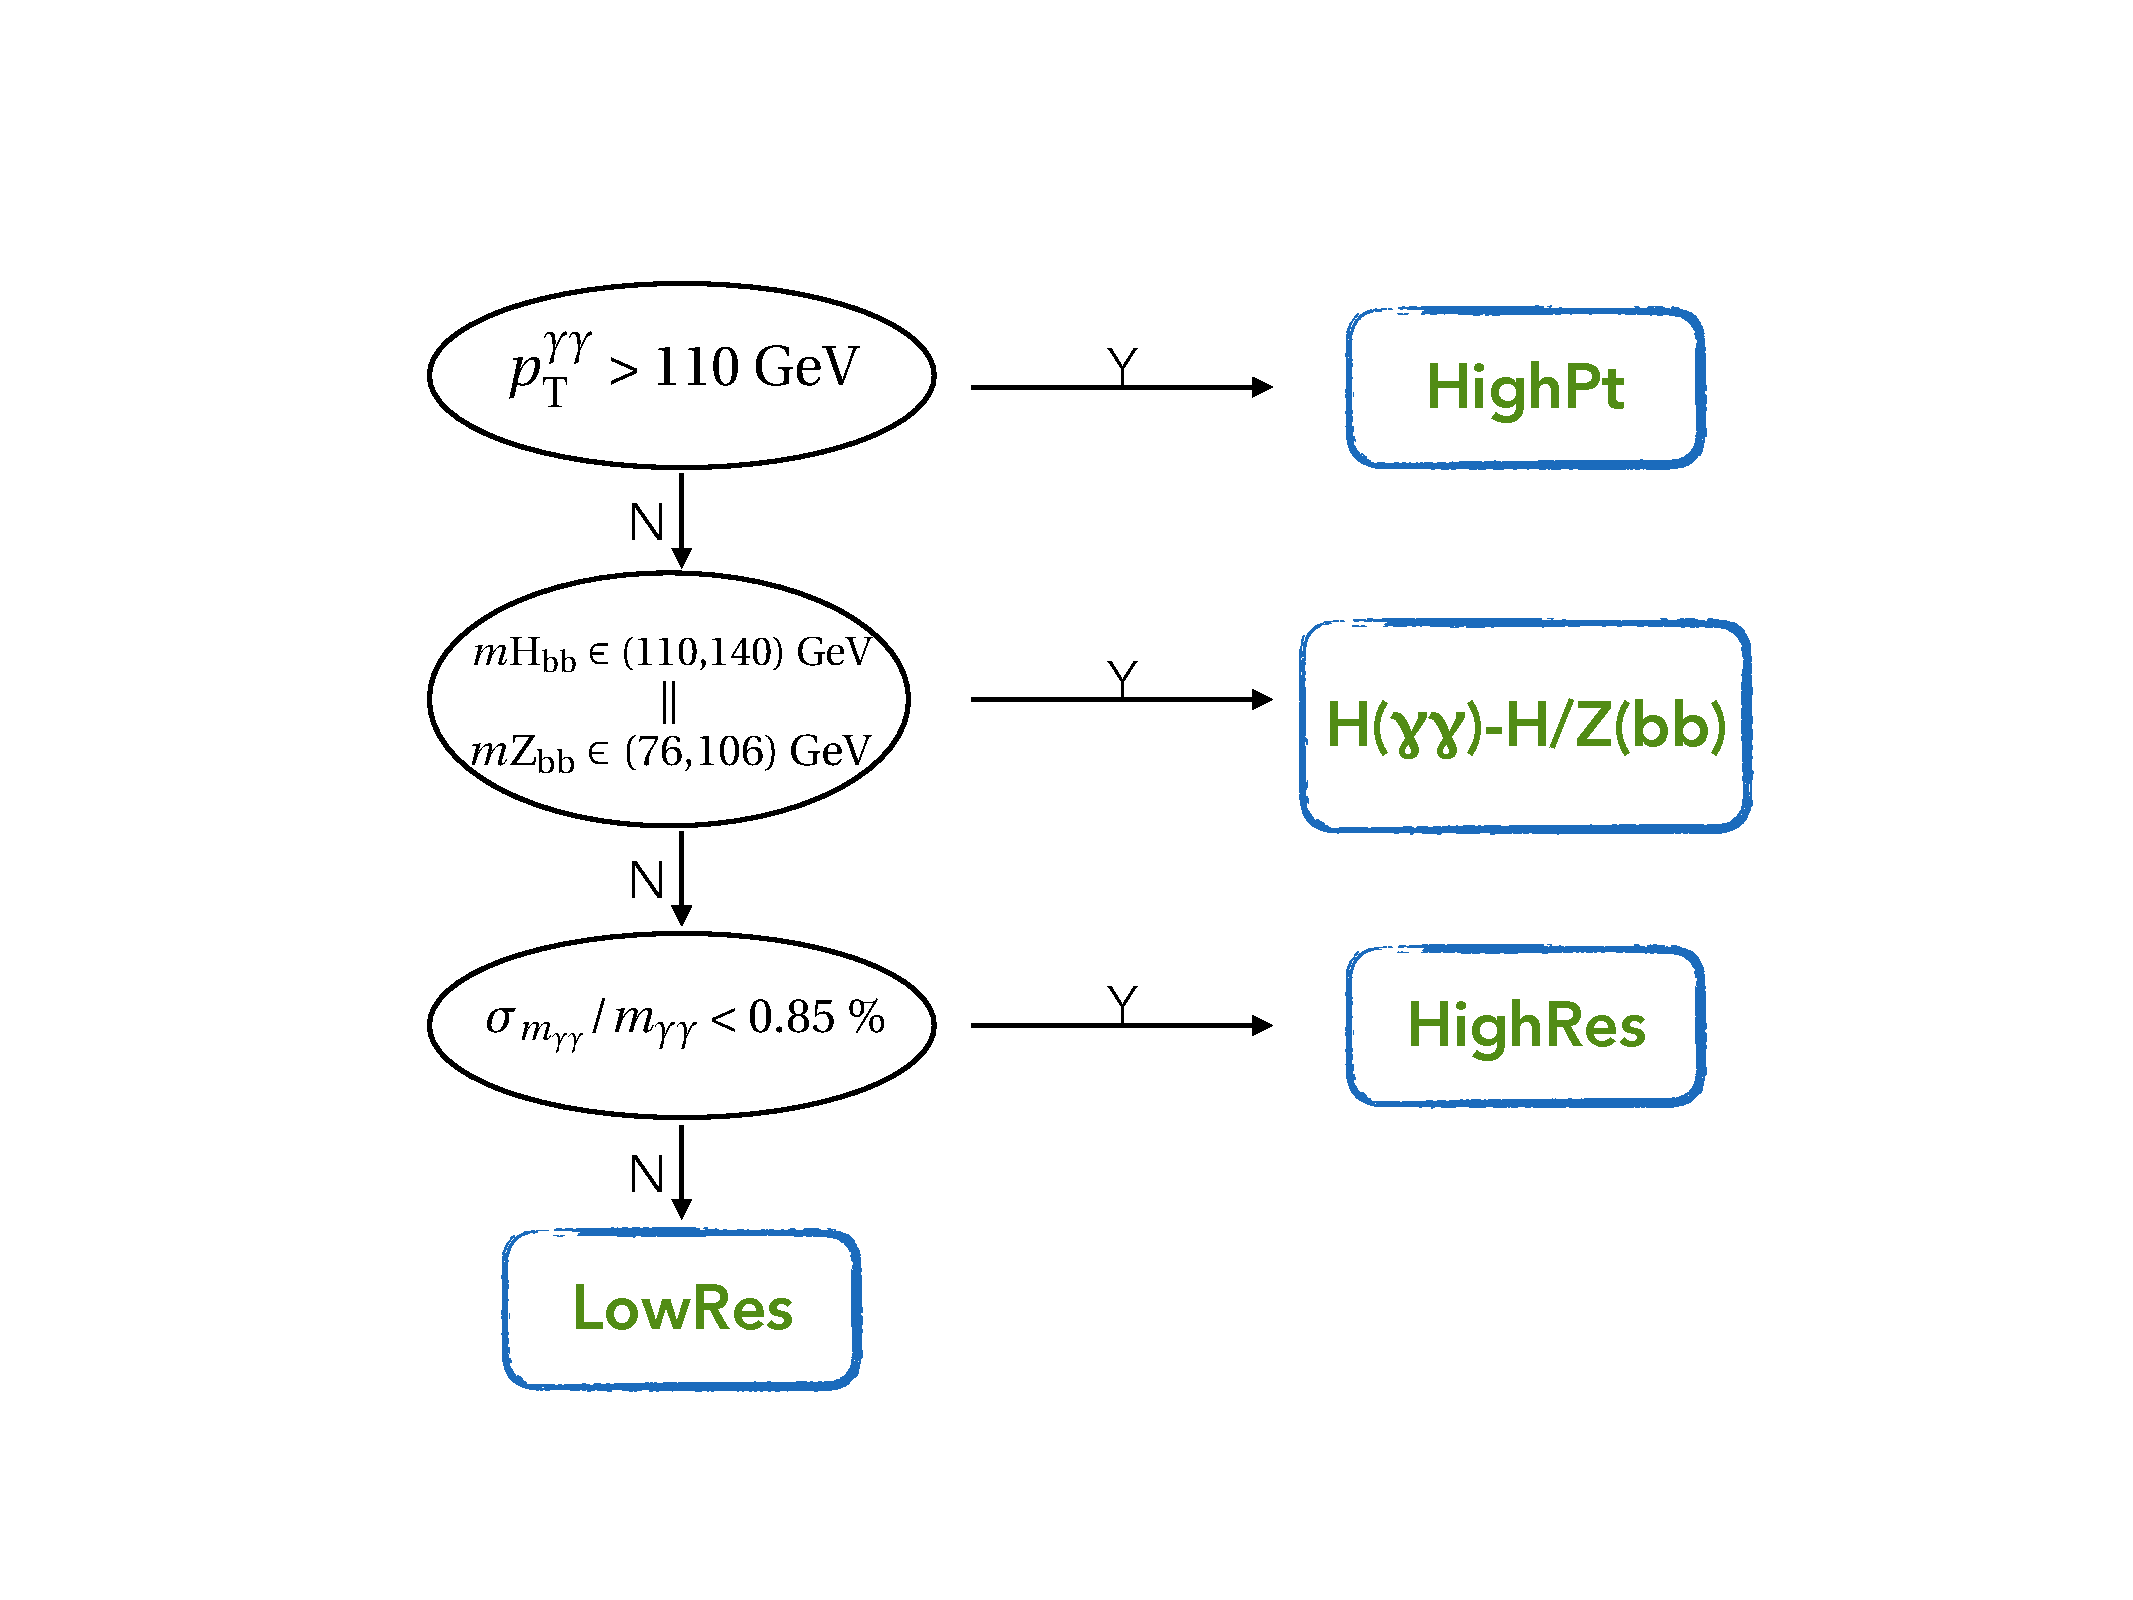
\includegraphics[width=0.75\textwidth,angle=0.]{figs/CategoriesDiagram_V2.pdf}\\
\caption{Diagram illustrating the event categorization used in the analysis.
\label{fig:categories}
}
\end{figure}


Each event category is divided into bins by rectangular cuts on
$M_{R}$ and $R^{2}$. The binning is chosen via an optimization procedure that uses 
the sbottom pair production simplified model discussed in Section~\ref{sec:intro}
as a benchmark model to determine the best bin boundaries. The algorithm begins with a
single bin covering the entire $M_{R}$-$R^{2}$ plane. A division is made in
either $M_{R}$ or $R^{2}$ at the value, which maximizes the expected statistical significance.  
This process is repeated on each newly created bin, and until convergence is achieved. Each bin returned by the algorithm is treated
as a separate analysis search region.  This procedure is not performed on the LowRes category; 
the binning in the LowRes category is instead taken to be the same as that in the HighRes category.
The definition of the individual search regions is summarized in 
Table~\ref{tab:binSummary}.


\begin{table*}[h]
\begin{center}
\topcaption{A summary of the search region bins in each category is presented. 
The functional form used to model the non-resonant background is also listed. An exponential 
function of the form $e^{-ax}$ is denoted as ``singleExp''; 
a modified exponential function of the form $e^{-ax^{b}}$  is denoted as ``modExp''; 
and an N'th order Bernstein polynomial is denoted by ``polyN''. }
\begin{tabular}{|c|c|c|c|c|}
\hline
Bin Number & Category & $M_{R}$ Bin & $R^{2}$ Bin              & Non-Resonant Bkg Model    \\ 
\hline
0          & HighPt &  600  - $\infty$ &   0.025 - $\infty$   & poly3         \\
1          & HighPt &  150  - 600    &   0.130 - $\infty$     & singleExp     \\
2          & HighPt &  1250 - $\infty$ &   0.000 - 0.025      & poly2         \\
3          & HighPt &  150  - 450    &   0.000 - 0.130        & poly2         \\
4          & HighPt &  450  - 600    &   0.000 - 0.035        & singleExp     \\
5          & HighPt &  450  - 600    &   0.035 - 0.130        & singleExp     \\
6          & HighPt &  600  - 1250   &   0.000 - 0.015        & singleExp     \\
7          & HighPt &  600  - 1250   &   0.015 - 0.025        & singleExp     \\
\hline
8          & H($\gamma\gamma$)-H/Z(bb)   &  150 - $\infty$ &   0.000 - $\infty$    & singleExp     \\
\hline
9          & HighRes & 150 - 250     &   0.000 - 0.175        & modExp        \\
10         & HighRes & 150 - 250     &   0.175 - $\infty$     & singleExp     \\
11         & HighRes & 250 - $\infty$  &   0.05  - $\infty$   & singleExp     \\
12         & HighRes & 250 - 600     &   0.000 - 0.05         & modExp        \\
13         & HighRes & 600 - $\infty$  &   0.000 - 0.05       & singleExp     \\
\hline
9          & LowRes & 150 - 250     &   0.000 - 0.175         & modExp        \\
10         & LowRes & 150 - 250     &   0.175 - $\infty$      & singleExp     \\
11         & LowRes & 250 - $\infty$  &   0.05  - $\infty$    & modExp        \\
12         & LowRes & 250 - 600     &   0.000 - 0.05          & modExp        \\
13         & LowRes & 600 - $\infty$  &   0.000 - 0.05        & singleExp     \\
\hline
\end{tabular}
\label{tab:binSummary}
\end{center}
\end{table*}


To illustrate how events from a typical SUSY signal might be distributed in these
bins, the distribution of events in the $M_{R}$ and $R^{2}$ plane for 
the sbottom pair production signal model discussed in Section~\ref{sec:intro}
is shown in Figures~\ref{fig:SignalModelMRRsq_HighPt}~and~\ref{fig:SignalModelMRRsq_HighResLowRes}
for the HighPt, HighRes, and LowRes categories, respectively.

\begin{figure}[ht!]
\centering
 \begin{tabular}{cc}
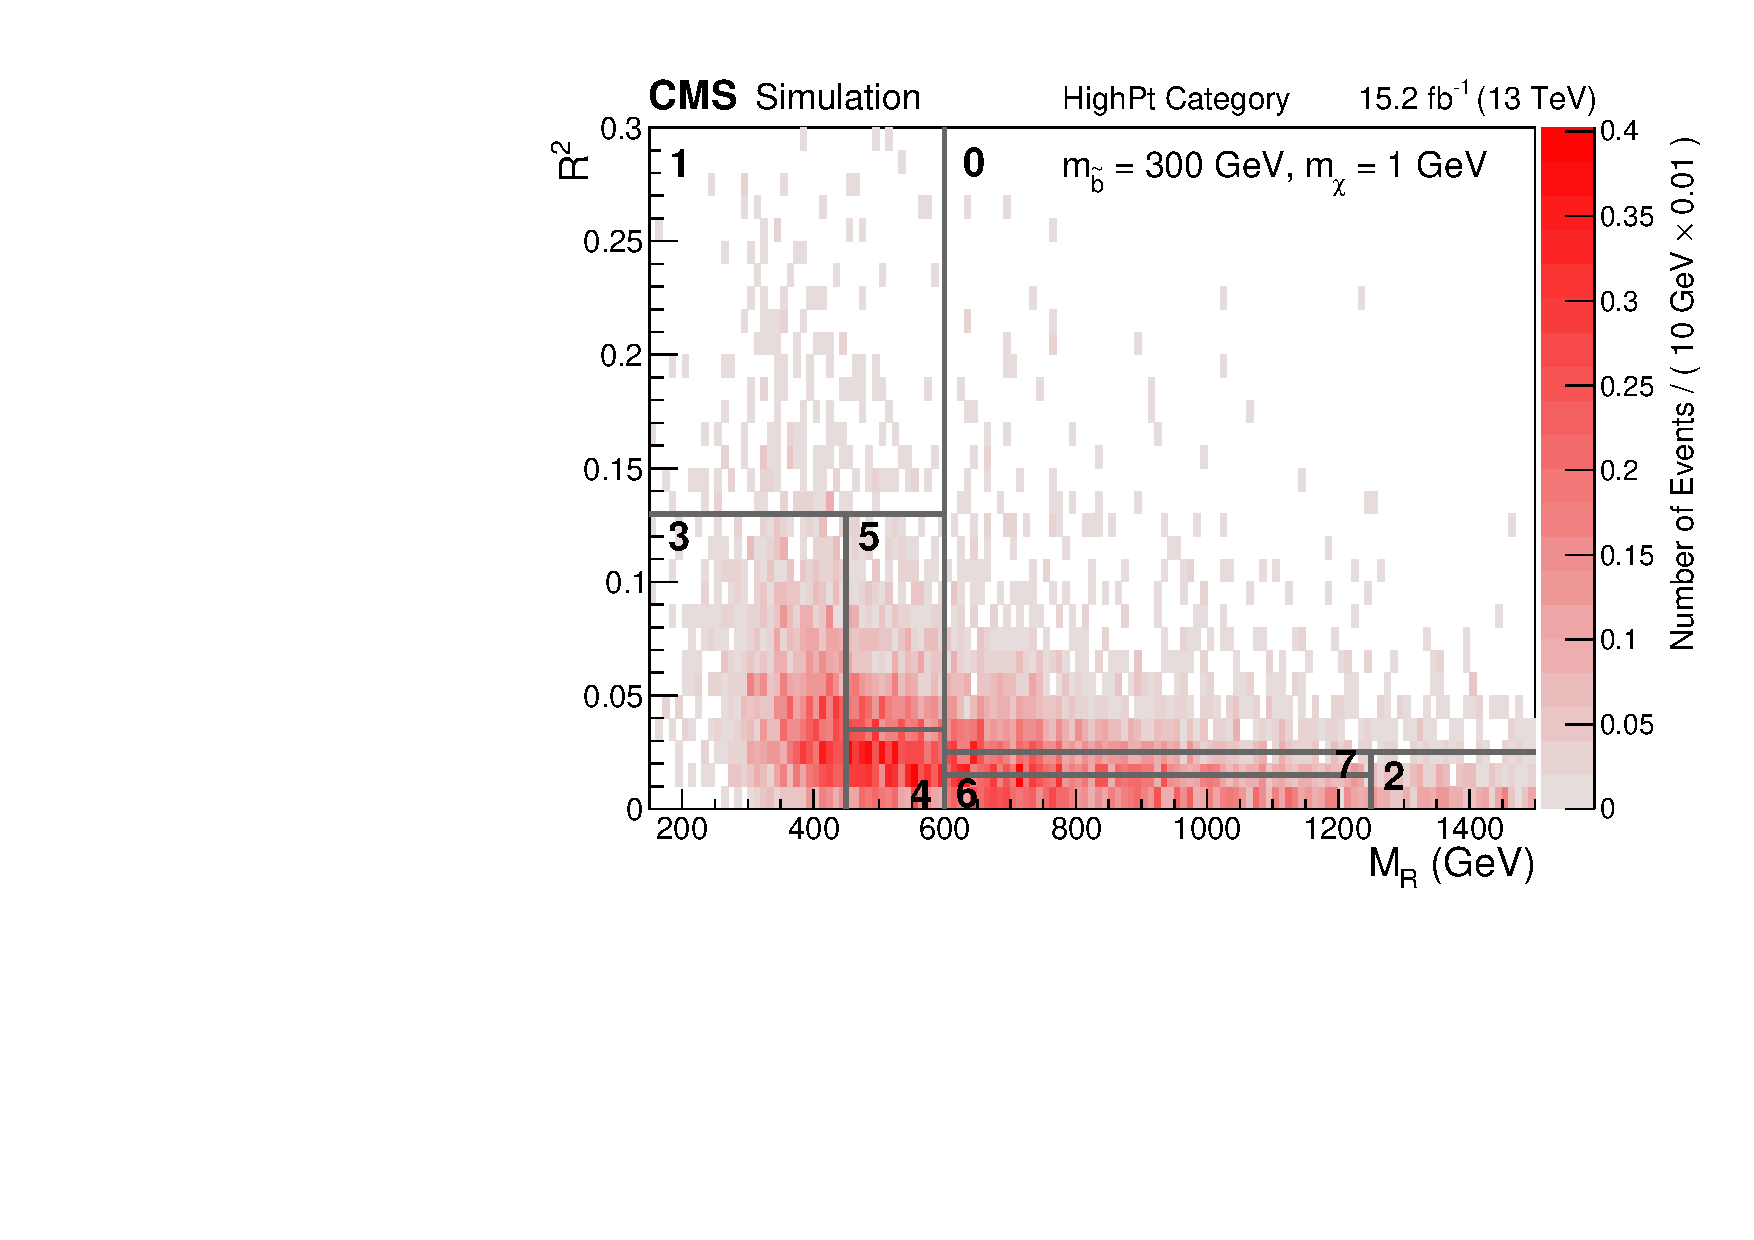
\includegraphics[width=0.49\textwidth, angle=0.]{figs/SignalT2BH_300_1_MRRsq_highpt.pdf}  & 
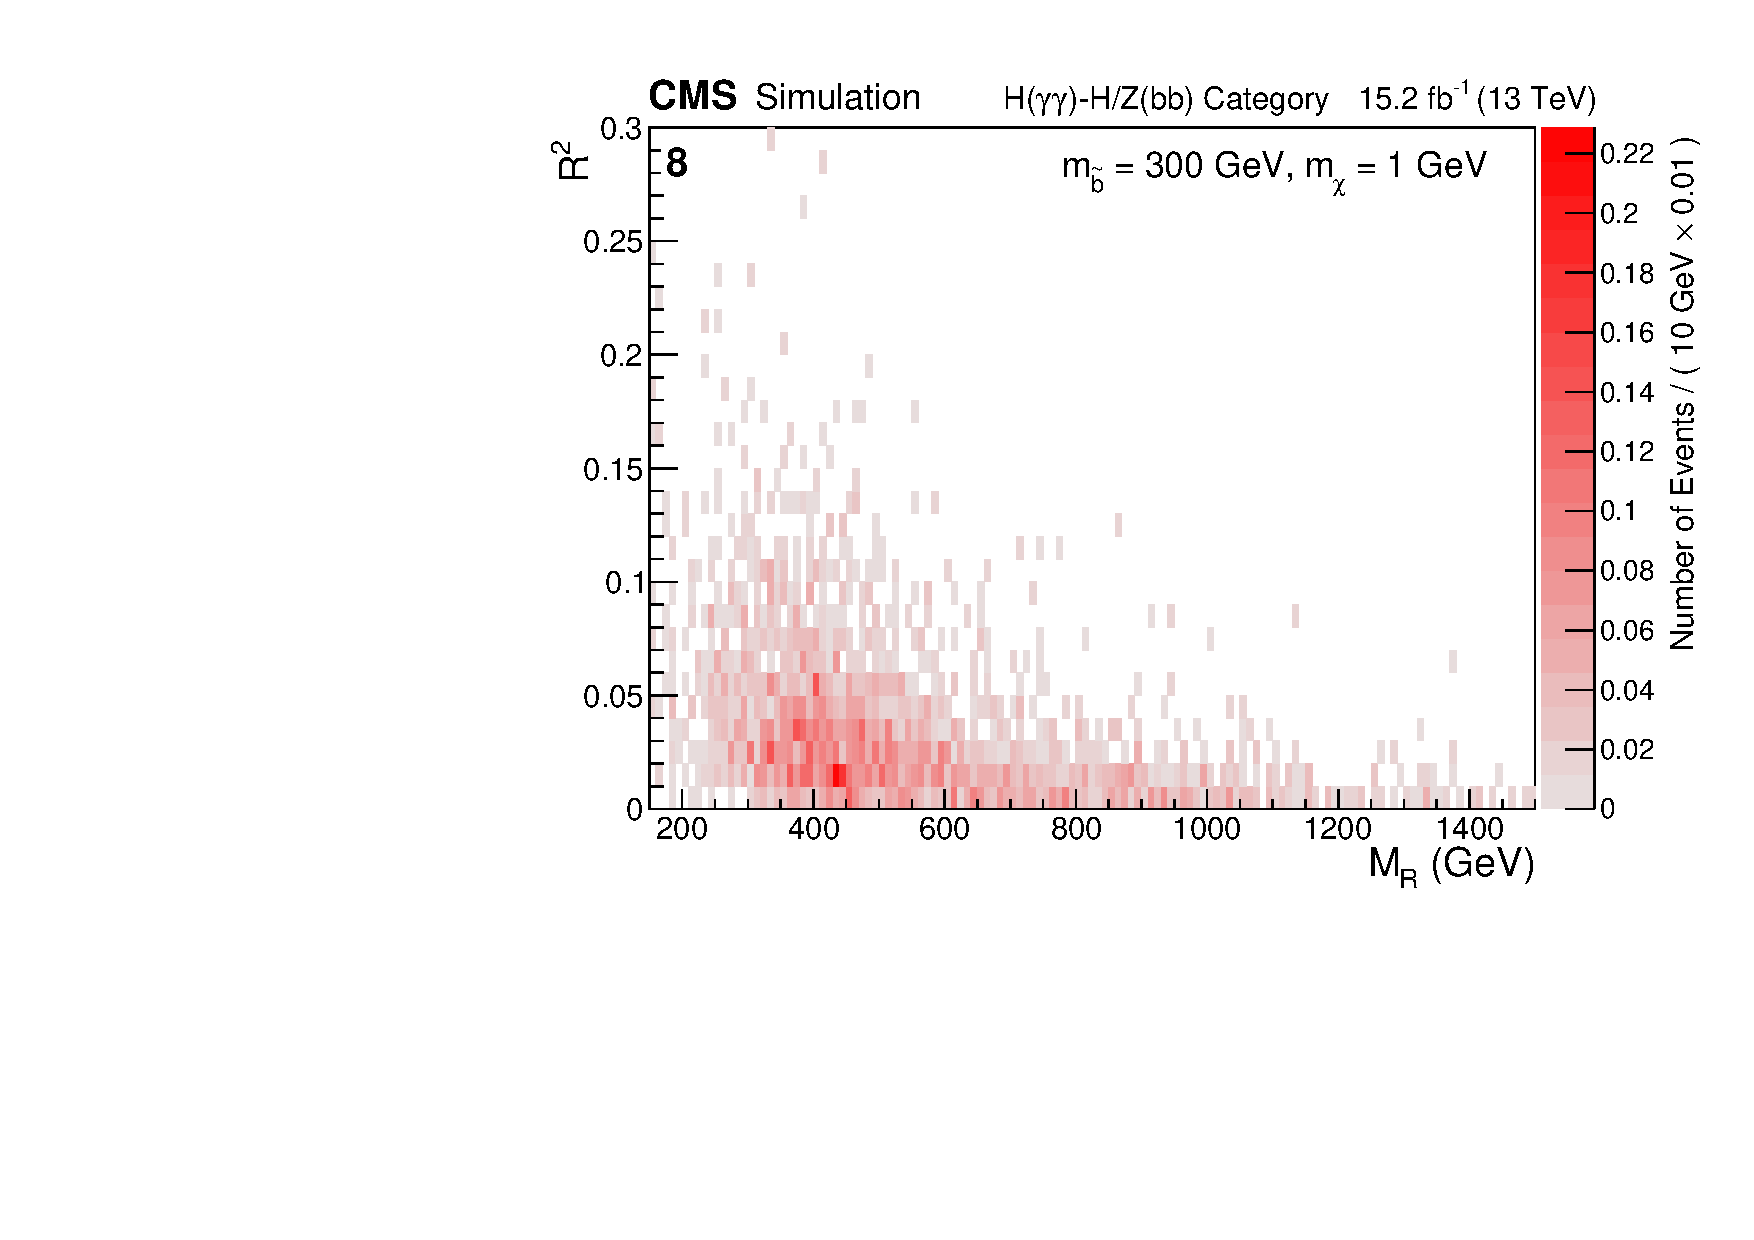
\includegraphics[width=0.49\textwidth, angle=0.]{figs/SignalT2BH_300_1_MRRsq_hzbb.pdf}  
\end{tabular}
\caption{ Distribution of events in the $M_{R}$ and $R^{2}$ plane for the HighPt and
H($\gamma\gamma$)-H/Z(bb) category for sbottom pair production with 
$m_{\tilde{b}}=300$~GeV and $m_{\chi}=1$~GeV. The signal expectation is shown in the
color scale and the bin numbers show where each bin is located in the $M_{R}$ and $R^{2}$ plane. 
\label{fig:SignalModelMRRsq_HighPt}}
\end{figure}

\begin{figure}[ht!]
\centering
 \begin{tabular}{cc}
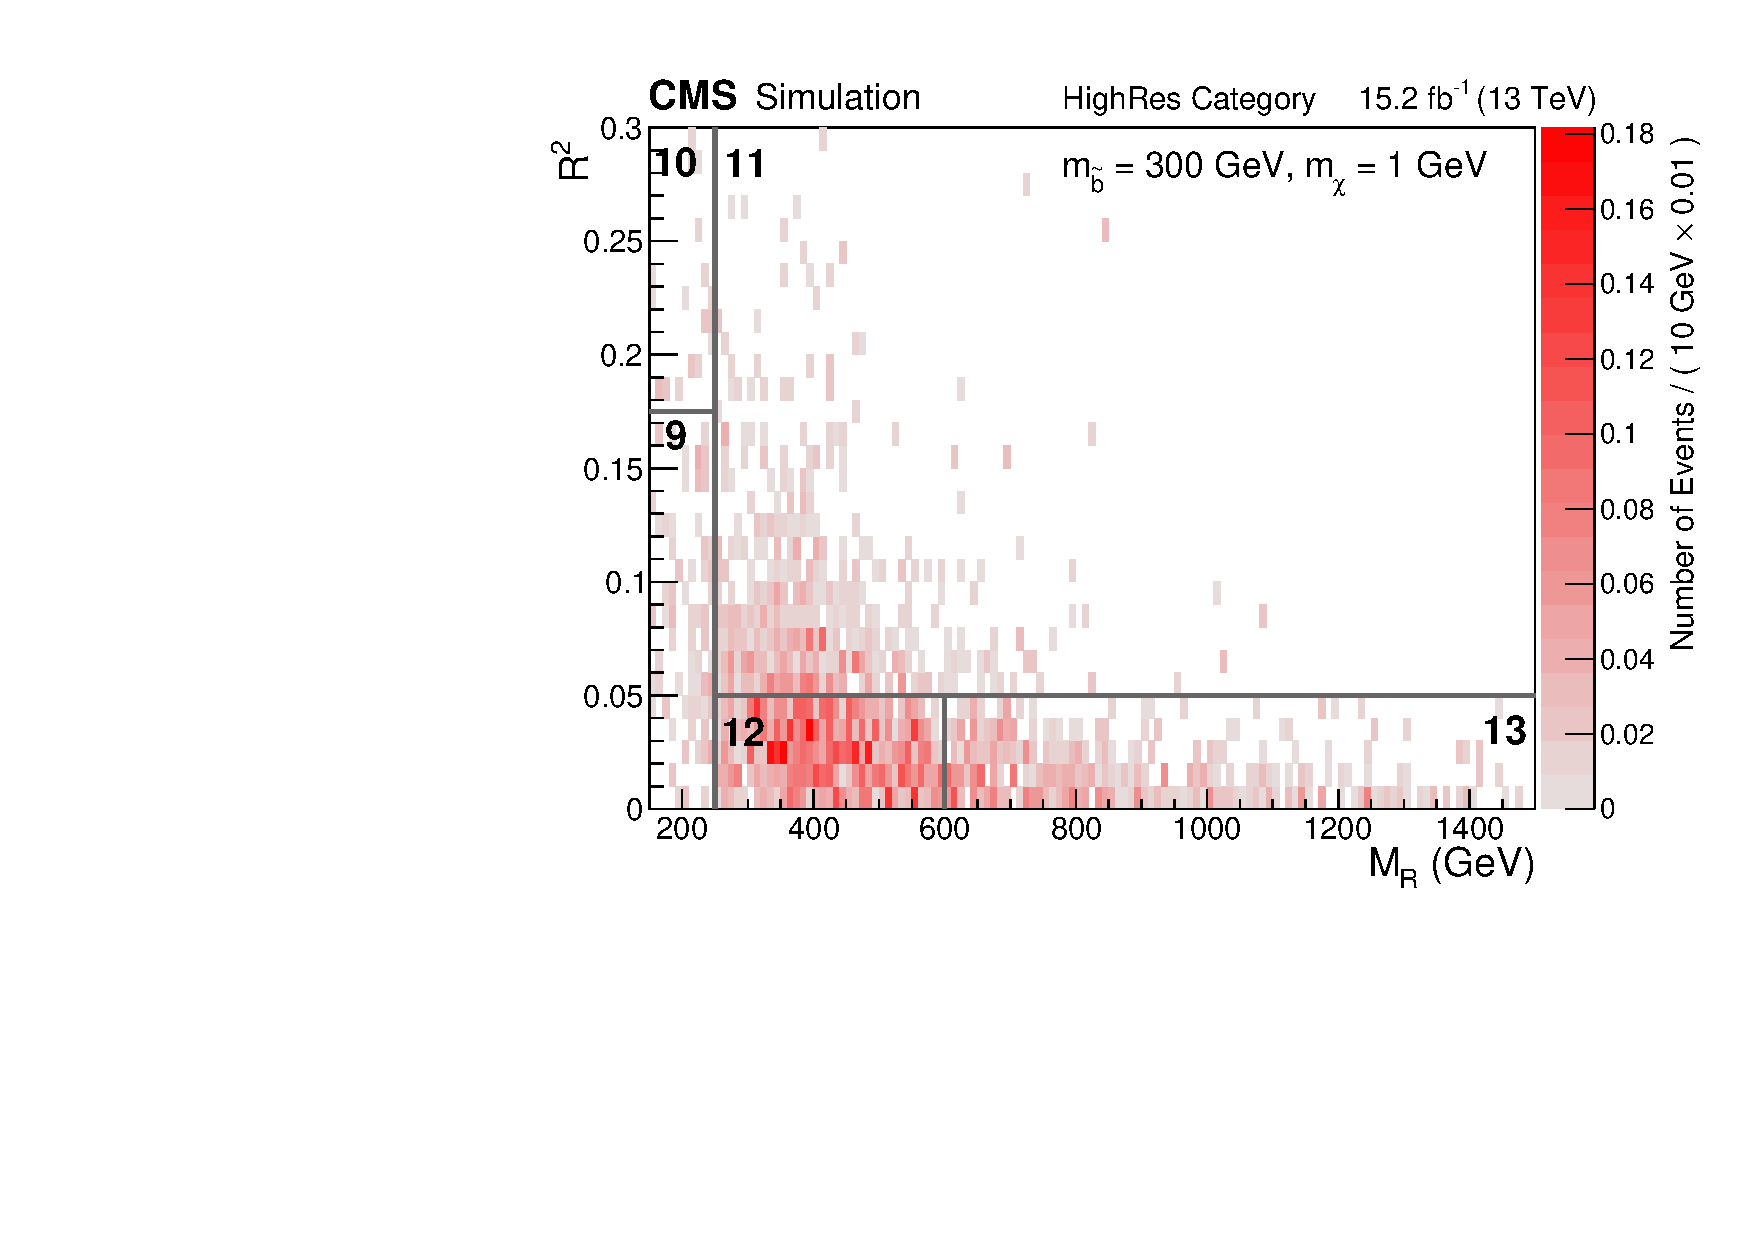
\includegraphics[width=0.49\textwidth, angle=0.]{figs/SignalT2BH_300_1_MRRsq_highres.pdf}  & 
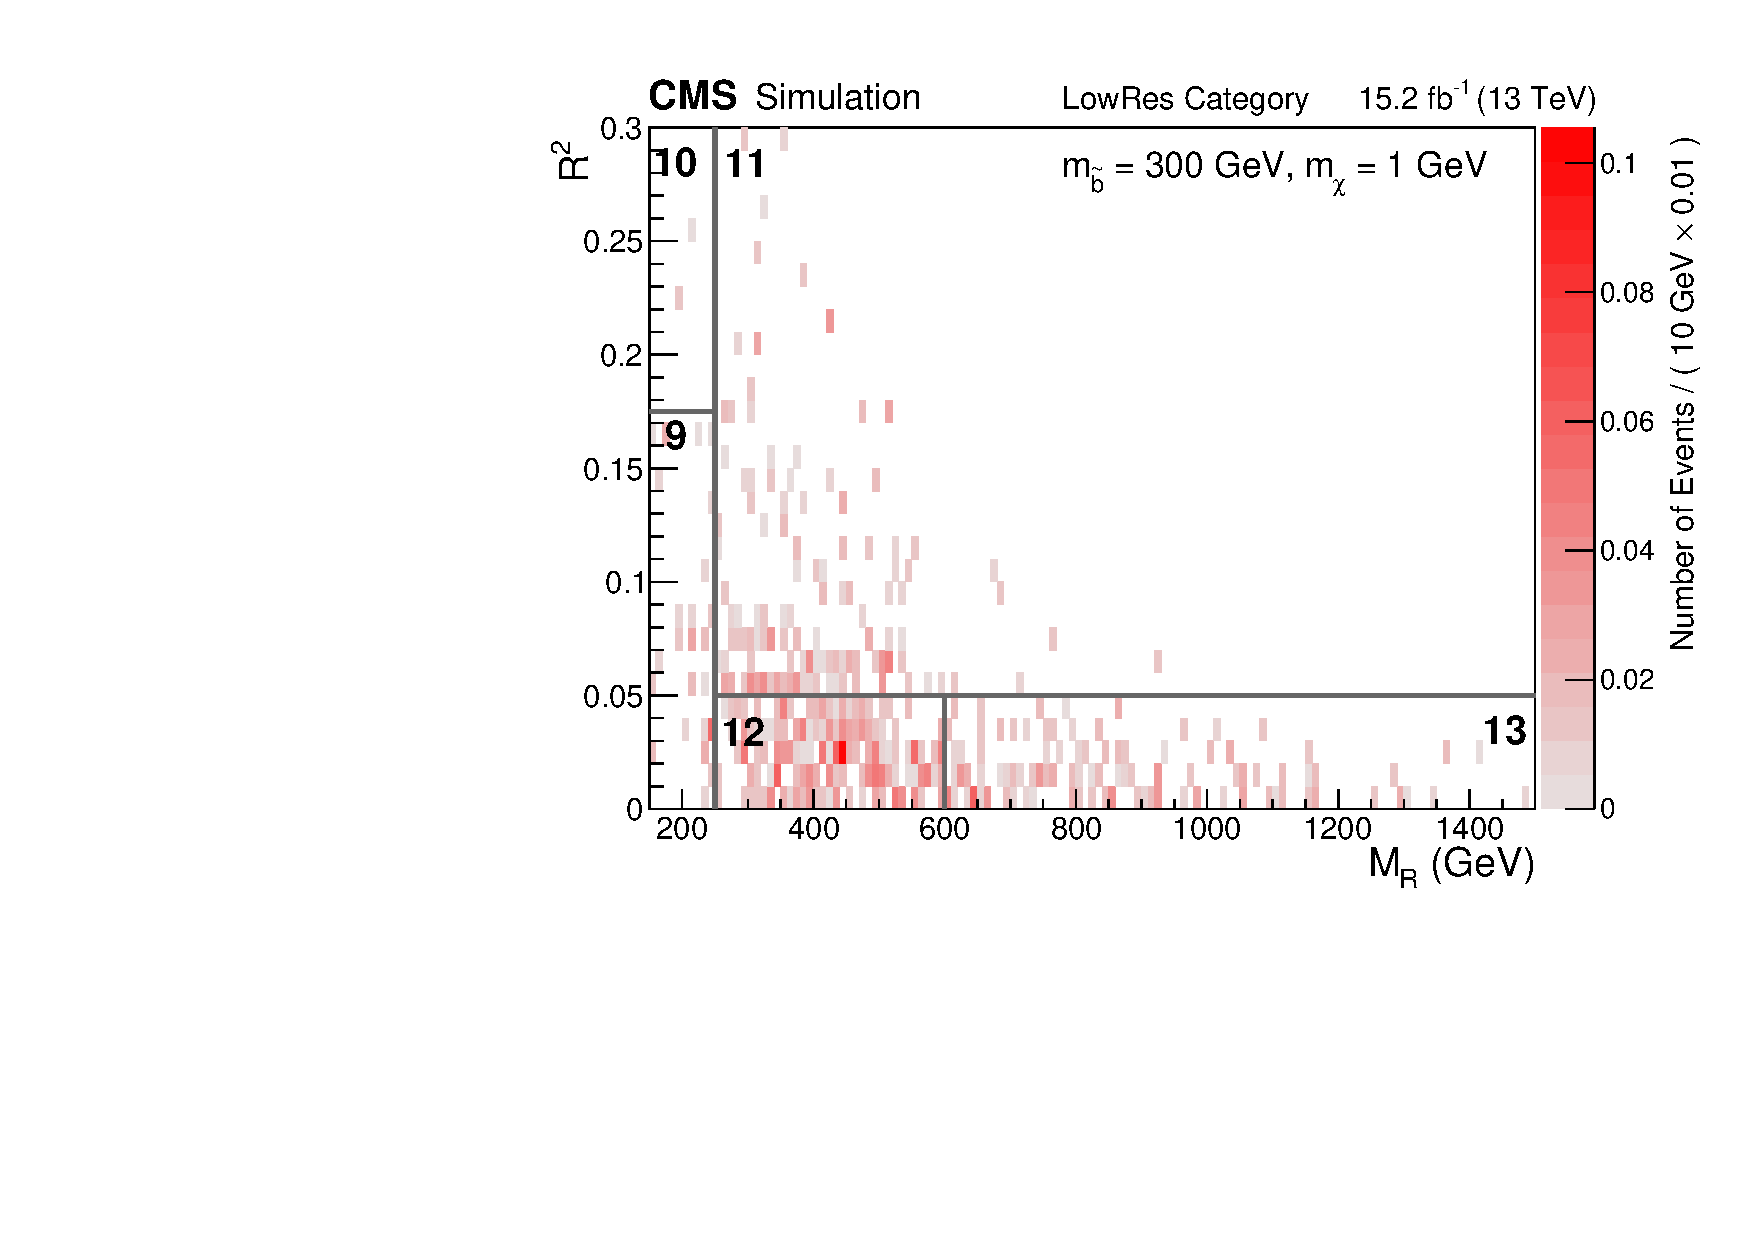
\includegraphics[width=0.49\textwidth, angle=0.]{figs/SignalT2BH_300_1_MRRsq_lowres.pdf}  
\end{tabular}
\caption{ Distribution of events in the $M_{R}$ and $R^{2}$ plane for the HighRes and LowRes categories
for sbottom pair production with $m_{\tilde{b}}=300$~GeV and $m_{\chi}=1$~GeV. 
The signal expectation is shown in the
color scale and the bin numbers show where each bin is located in the $M_{R}$ and $R^{2}$ plane. 
\label{fig:SignalModelMRRsq_HighResLowRes}}
\end{figure}



\section{Background Estimation}\label{sec:bkg}

Within each search bin, we extract a potential signal by fitting to the
diphoton mass spectrum. There are two types of backgrounds: 
a non-resonant background that is primarily due to QCD production
of two photons or one photon and one jet, and a resonant background
from standard model Higgs production. The non-resonant background
is modeled with the functional form given in Table~\ref{tab:binSummary}
for each individual search region bin, and all parameters of
the function are unconstrained in the fit. The functional form model
for each search region bin is selected on the basis of its Akaike 
Information Criterion (AIC) score~\cite{AIC}, as well as tests of
fit biases for a set of alternative models that all describe the 
data in the sideband well. 

The standard model Higgs background and the SUSY signal are each
modeled with a double-sided crystal ball function
fit to the diphoton mass distribution obtained from the Monte Carlo simulation.
The parameters of each double-sided crystal ball function are held constant in the signal extraction procedure, 
with the exception of the parameter that determines the location of the peak. This parameter is allowed to float
but is restricted via a Gaussian constraint to the region around the Higgs mass.
The width of the Gaussian constraint is $1\%$, corresponding to the systematic uncertainty on the photon energy 
scale.

The normalization of the standard model Higgs background in each bin 
is predicted from the Monte Carlo simulation, and is constrained 
to that value in the fit within uncertainties.
Signal yields are also predicted from the Monte Carlo simulation. 

Each bin in the HighRes category is fit simultaneously with the corresponding bin in the LowRes category.
The relative SM Higgs and SUSY signal yields in the two categories are constrained according to 
the simulation prediction. The ratio of the yields in the HighRes and LowRes
categories is expected to be independent of the signal model and background
process.

Nuisance parameters for various theoretical and instrumental uncertainties that
can affect the SM Higgs and signal normalization and are profiled to propagate systematic uncertainties.
A more detailed discussion of systematic uncertainties can be found below in 
Section~\ref{sec:systematics}. The Monte Carlo simulation predictions for the standard model Higgs background
normalization are shown in Table~\ref{tab:SMHBkgPrediction} for each search region
bin. 

%% \begin{table*}[htb]
%% \begin{center}
%% \caption{The predicted yields for the standard model Higgs background are shown for an integrated luminosity 
%% corresponding to 15.2~$\mathrm{fb}^{-1}$ for each search region considered in this analysis. 
%% The uncertainties shown account for Monte Carlo statistical uncertainties only.
%% \label{tab:SMHBkgPrediction}
%% }
%% \def\arraystretch{1.5}
%% \begin{tabular}{|c|c|c|c|c|c|c|}
%% \hline
%%     & & \multicolumn{4}{c|}{Expected SM Higgs Yield} \\
%% \hline
%% Bin & Category & ggH & $t\bar{t}$H & VBF H & VH & bbH  \\
%% \small
%% \hline
%% 0  & HighPt & 1.117 $\pm$ 0.082 & 0.494 $\pm$ 0.019 & 0.177 $\pm$ 0.010 & 0.256 $\pm$ 0.018 & 0.009 $\pm$ 0.002    \\
%% 1  & HighPt & 0.485 $\pm$ 0.049 & 0.219 $\pm$ 0.011 & 0.071 $\pm$ 0.007 & 0.606 $\pm$ 0.026 & 0.006 $\pm$ 0.002     \\
%% 2  & HighPt & 1.738 $\pm$ 0.108 & 0.231 $\pm$ 0.013 & 0.875 $\pm$ 0.023 & 0.066 $\pm$ 0.011 & 0.017 $\pm$ 0.004     \\
%% 3  & HighPt & 20.540 $\pm$ 0.317 & 0.378 $\pm$ 0.014 & 3.976 $\pm$ 0.049 & 2.322 $\pm$ 0.049 & 0.160 $\pm$ 0.011    \\
%% 4  & HighPt & 6.154 $\pm$ 0.185 & 0.188 $\pm$ 0.011 & 1.735 $\pm$ 0.032 & 0.437 $\pm$ 0.023 & 0.057 $\pm$ 0.006     \\
%% 5  & HighPt & 1.130 $\pm$ 0.073 & 0.228 $\pm$ 0.012 & 0.183 $\pm$ 0.010 & 0.194 $\pm$ 0.016 & 0.012 $\pm$ 0.003     \\
%% 6  & HighPt & 6.947 $\pm$ 0.202 & 0.278 $\pm$ 0.015 & 2.856 $\pm$ 0.041 & 0.280 $\pm$ 0.021 & 0.050 $\pm$ 0.007     \\
%% 7  & HighPt & 1.963 $\pm$ 0.103 & 0.189 $\pm$ 0.011 & 0.375 $\pm$ 0.015 & 0.171 $\pm$ 0.015 & 0.008 $\pm$ 0.003     \\
%% \hline
%% 8  & H($\gamma\gamma$)-H/Z(bb)   & 0.362 $\pm$ 0.044 & 0.510 $\pm$ 0.017 & 0.032 $\pm$ 0.005 & 0.104 $\pm$ 0.011 & 0.059 $\pm$ 0.007   \\
%% \hline
%% 9  & HighRes & 27.191 $\pm$ 0.342 & 0.094 $\pm$ 0.007 & 3.413 $\pm$ 0.046 & 1.930 $\pm$ 0.043 & 0.419 $\pm$ 0.018    \\   
%% 10 & HighRes & 0.274 $\pm$ 0.035 & 0.054 $\pm$ 0.006 & 0.045 $\pm$ 0.005 & 0.204 $\pm$ 0.014 & 0.005 $\pm$ 0.002   \\     
%% 11 & HighRes & 0.984 $\pm$ 0.064 & 0.332 $\pm$ 0.014 & 0.217 $\pm$ 0.011 & 0.194 $\pm$ 0.017 & 0.046 $\pm$ 0.006    \\    
%% 12 & HighRes & 15.992 $\pm$ 0.282 & 0.295 $\pm$ 0.013 & 3.908 $\pm$ 0.049 & 0.630 $\pm$ 0.029 & 0.387 $\pm$ 0.018   \\   
%% 13 & HighRes & 1.805 $\pm$ 0.100 & 0.222 $\pm$ 0.012 & 1.220 $\pm$ 0.028 & 0.094 $\pm$ 0.013 & 0.086 $\pm$ 0.010   \\    
%% \hline
%% 9  & LowRes & 9.642 $\pm$ 0.198 & 0.041 $\pm$ 0.004 & 1.176 $\pm$ 0.026 & 0.725 $\pm$ 0.025 & 0.142 $\pm$ 0.011    \\
%% 10 & LowRes & 0.128 $\pm$ 0.020 & 0.022 $\pm$ 0.003 & 0.008 $\pm$ 0.003 & 0.066 $\pm$ 0.009 & 0.002 $\pm$ 0.001    \\
%% 11 & LowRes & 0.320 $\pm$ 0.040 & 0.114 $\pm$ 0.008 & 0.067 $\pm$ 0.007 & 0.084 $\pm$ 0.010 & 0.017 $\pm$ 0.004    \\
%% 12 & LowRes & 6.027 $\pm$ 0.174 & 0.110 $\pm$ 0.008 & 1.459 $\pm$ 0.029 & 0.245 $\pm$ 0.018 & 0.121 $\pm$ 0.011    \\
%% 13 & LowRes & 0.842 $\pm$ 0.064 & 0.089 $\pm$ 0.007 & 0.456 $\pm$ 0.017 & 0.042 $\pm$ 0.008 & 0.026 $\pm$ 0.006    \\
%% \hline
%% \end{tabular}
%% \end{center}
%% \end{table*}


\begin{table*}[htb]
\begin{center}
\caption{The predicted yields for the standard model Higgs background processes 
are shown for an integrated luminosity corresponding to 15.2~$\mathrm{fb}^{-1}$ for 
each search region considered in this analysis. The contributions from 
each standard model Higgs process is shown separately, and the total 
is shown on the rightmost column along with its full uncertainty.
\label{tab:SMHBkgPrediction}
}
\def\arraystretch{1.5}
\begin{tabular}{|c|c|c|c|c|c|c|c|}
\hline
    & & \multicolumn{5}{c|}{Expected SM Higgs Yield} & \\
\hline
\small
Bin & Category & ggH & $t\bar{t}$H & VBF H & VH & bbH & Total \\
%\small
\hline
0  & HighPt & 1.09   & 0.49   & 0.17   & 0.25   & 0.01    & 2.0 $\pm$ 0.4    \\
1  & HighPt & 0.45   & 0.22   & 0.07   & 0.60   & 0.00    & 1.4 $\pm$ 0.3    \\
2  & HighPt & 1.75   & 0.23   & 0.89   & 0.07   & 0.02    & 3.0 $\pm$ 0.6    \\ 
3  & HighPt & 20.82  & 0.38   & 4.05   & 2.36   & 0.16    & 27.7 $\pm$ 8.0  \\ 
4  & HighPt & 6.30   & 0.20   & 1.77   & 0.45   & 0.06    & 8.8 $\pm$ 2.5    \\
5  & HighPt & 1.09   & 0.23   & 0.18   & 0.19   & 0.01    & 1.7 $\pm$ 0.4    \\
6  & HighPt & 7.15   & 0.21   & 2.91   & 0.28   & 0.05    & 10.7 $\pm$ 2.7   \\
7  & HighPt & 1.94   & 0.19   & 0.37   & 0.17   & 0.01    & 2.7 $\pm$ 0.8    \\
\hline                                                                     
8  & H($\gamma\gamma$)-H/Z(bb)   & 0.35   & 0.51   & 0.03   & 0.10   & 0.06    & 1.0 $\pm$ 0.2    \\
\hline                                                                     
9  & HighRes & 27.57 & 0.10   & 3.49   & 1.97   & 0.43    & 33.5 $\pm$ 10.4  \\   
10 & HighRes & 0.26  & 0.06   & 0.04   & 0.20   & 0.01    & 0.6 $\pm$ 0.1    \\     
11 & HighRes & 0.94  & 0.33   & 0.21   & 0.19   & 0.05    & 1.7 $\pm$ 0.4    \\    
12 & HighRes & 16.16 & 0.31   & 3.99   & 0.64   & 0.39    & 21.5 $\pm$ 5.4   \\   
13 & HighRes & 1.83  & 0.23   & 1.25   & 0.10   & 0.09    & 3.5 $\pm$ 1.0    \\    
\hline                                                                     
9  & LowRes & 9.55   & 0.039  & 1.18   & 0.72   & 0.14    & 11.6 $\pm$ 3.8   \\
10 & LowRes & 0.12   & 0.02   & 0.01   & 0.07   & 0.00    & 0.2 $\pm$ 0.1    \\
11 & LowRes & 0.32   & 0.11   & 0.06   & 0.08   & 0.02    & 0.6 $\pm$ 0.2    \\
12 & LowRes & 6.02   & 0.11   & 1.46   & 0.24   & 0.12    & 7.9 $\pm$ 2.3    \\
13 & LowRes & 0.82   & 0.09   & 0.46   & 0.04   & 0.03    & 1.4 $\pm$ 0.4    \\
\hline
\end{tabular}
\end{center}
\end{table*}



\section{Nos-resonant Background Functional Form Selection: AIC
  Criterion and Bias Tests}
For each signal region -- i.e. every \MR-\Rtwo bin in the search -- a functional form is needed to estimate the non-resonant
contribution from SM QCD  production. This selection process has two
steps: 1) the AIC criterion, and 2) the bias test.

The AIC criterion step is used to decide what functions described
reasonable well the observed data and therefore describe better the
QCD background in each signal region. The AIC criterion, first
introduced by Akaike in 1973~\cite{AIC}, is an estimate of the
Kullback–Leibler divergence~\cite{kullback1951} -- the later is a measure of
the distance between two probability density functions. Therefore the
AIC criterion is a measure of the distance between the data and a
particular probability density function (p.d.f). An advantage over
other goodness of fit quantities is that the AIC criterion also
accounts for the fact that a function may have move free parameters
and thus more flexibility to accomodate the observed data. It is
useful to define the AIC score:
\begin{equation}
\label{eq:AIC}
\mathrm{AIC}_{i} = -2log(\mathcal{L}) + 2k -\frac{2k(k+1)}{n-k-1},
\end{equation}

where $i$ represents the $i$-th p.d.f under study, $\mathcal{L}$ is the likelihood after the minimization process,
k is the number of free parameters of the p.d.f, and n is the total
numer of observed events. The procedure is as follows: from a set of
functions, all AIC scores are computed, then AIC score differences
with respect ot the minumum AIC score
($\Delta_{i} = \mathrm{AIC}_{i} -\mathrm{AIC_{min}}$) are calculated.
%for all the functions but the one with the minumum AIC score -- by
%construction its $\mathrm{AIC_{s}}$ is zero.
The AIC weight, which could be interpreted as the probability that the
p.d.f under study is the true p.d.f from were the observed
dataset was draw, is defined as
\begin{equation}
\label{eq:AICweight}
\omega_{i} = \frac{e^{-\frac{1}{2}\Delta_{i}}}{\sum\limits_{j=0}^{7}e^{-\frac{1}{2}\Delta_{j}}}.
\end{equation}
Only p.d.fs with AIC weight larger than 0.1 pass the first step and
are then tested for the bias test described
below. Table~\ref{table:aicpdfs} shows the full list of p.d.fs used in
these studies. Tables~\ref{tab:AICresults1},~\ref{tab:AICresults2},~\ref{tab:AICresults3},  and
~\ref{tab:AICresults4} summarize four examples of the AIC results
obtained for four search regions -- one per each
category in the analysis --, Figures ~\ref{fig:AICresults1},~\ref{fig:AICresults2},~\ref{fig:AICresults3}, and
~\ref{fig:AICresults4} show the corresponding fits to the observed
data. It is of note that the AIC fits are done only to the
$m_{\gamma\gamma}\in \{[103-121],[129-160]\}$\GeV region.
\begin{table*}[h] 
\begin{center} 
\topcaption{Full list of p.d.f (function) used in the AIC test.} 
\footnotesize
\begin{tabular}{|c|c|c|} 
\hline
function name & short name & functional form\\
\hline
single exponential & singleExp & $e^{-\alpha m_{\gamma\gamma}}$\\
double exponential & doubleExp & $fe^{-\alpha_{1} m_{\gamma\gamma}}+(1-f)e^{-\alpha_{1} m_{\gamma\gamma}}$\\
single power law & singlePow & $m_{\gamma\gamma}^{-\alpha}$\\
double power law & doublePow &
                               $fm_{\gamma\gamma}^{-\alpha_{1}}+(1-f)m_{\gamma\gamma}^{-\alpha_{2}}$\\
modified exponential & modExp & $e^{-\alpha
                                m_{\gamma\gamma}^{\beta}}$\\
Bernstein polynomial order 2 & poly2 & $p_{0}(1-t)^{2} +
                                       p_{1}2t(1-t) + p_{2} t^{2}$\\
Bernstein polynomial order 3 & poly3 & $p_{0}(1-t)^{3} +
                                       p_{1}3t(1-t)^{2} + p_{2}3t^{2}(1-t)
                                       +p_{3} t^{3}$\\
Bernstein polynomial order 4 & poly4 & $p_{0}(1-t)^{4} +
                                       p_{1}4t(1-t)^{3} + p_{2}6t^{2}(1-t)^{2}
                                       +p_{3} 4t^{3}(1-t) + p_{4} t^{4}$\\
\hline
\end{tabular} 
\label{table:aicpdfs} 
\end{center} 
\end{table*} 

\begin{figure}[h] 
\begin{center} 
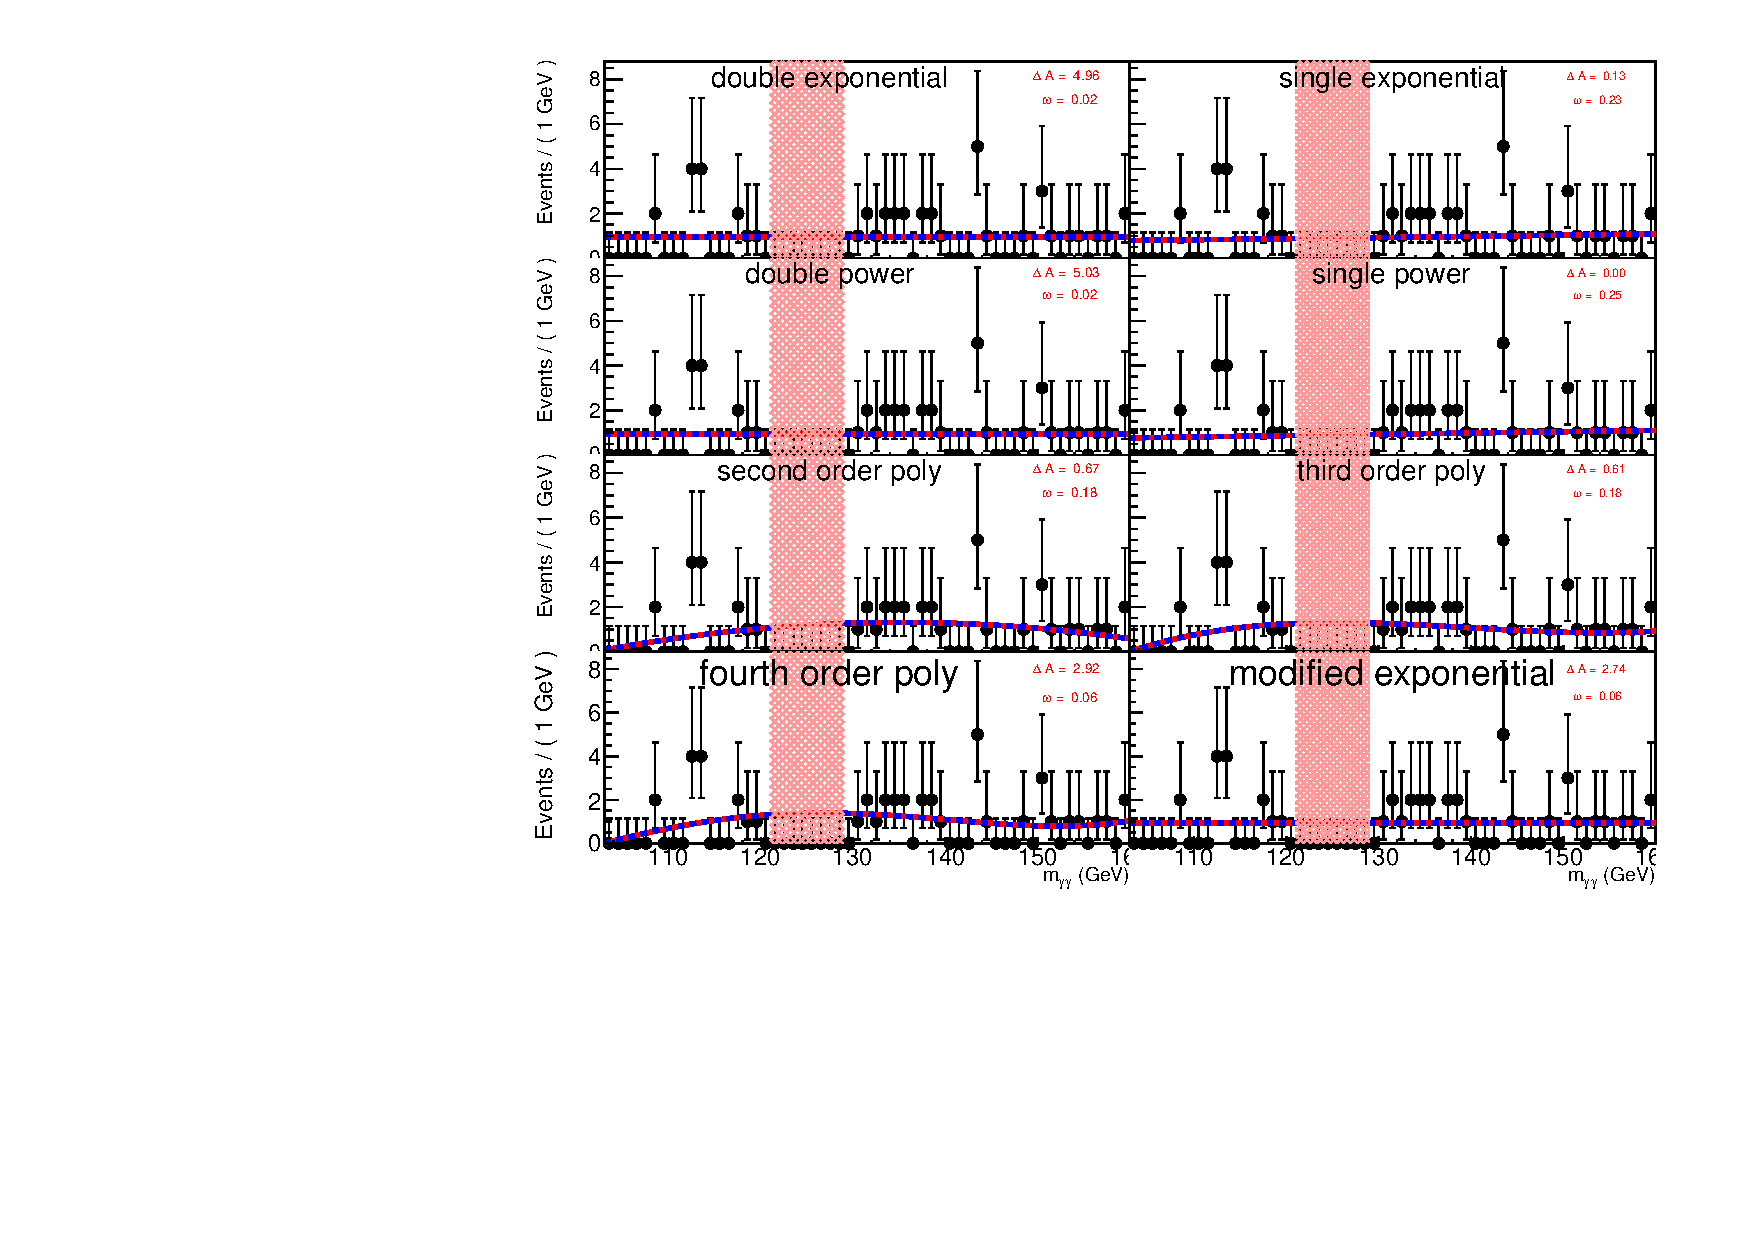
\includegraphics[width=0.6\textwidth]{hgg/highpt/600_0d025.pdf} 
\caption{sideband fits for the search region: HighPt, $M_R >
  600$\GeV , $R^2 > 0.025$.} 
\label{fig:AICresults1} 
\end{center} 
\end{figure} 

\begin{table*}[h] 
\begin{center} 
\topcaption{AIC results summary for the search region: HighPt, $M_R >
  600$\GeV , $R^2 > 0.025$.} 
\begin{tabular}{|c|c|ccc|c|} 
\hline function & \#P & $\Delta AIC$ & $\omega$ & $\omega_{max}/\omega$ & status \\ \hline 
\rowcolor[rgb]{0.31,0.78,0.47}  
singlePow &  1 &  0.000 &  0.247 &  1.000 &  0,  3 \\ 
\rowcolor[rgb]{0.31,0.78,0.47}  
singleExp &  1 &  0.128 &  0.232 &  1.066 &  0,  3 \\ 
\rowcolor[rgb]{0.31,0.78,0.47}  
poly3 &  4 &  0.605 &  0.183 &  1.353 &  0,  3 \\ 
\rowcolor[rgb]{0.31,0.78,0.47}  
poly2 &  3 &  0.673 &  0.177 &  1.400 &  0,  3 \\ 
\rowcolor[rgb]{1.0,0.41,0.38}  
modExp &  2 &  2.738 &  0.063 &  3.932 &  0,  3 \\ 
\rowcolor[rgb]{1.0,0.41,0.38}  
poly4 &  5 &  2.916 &  0.058 &  4.297 &  0,  3 \\ 
\rowcolor[rgb]{1.0,0.41,0.38}  
doubleExp &  3 &  4.958 &  0.021 & 11.929 &  0,  3 \\ 
\rowcolor[rgb]{1.0,0.41,0.38}  
doublePow &  3 &  5.031 &  0.020 & 12.371 &  0,  3 \\ 
\hline 
\end{tabular} 
\label{tab:AICresults1} 
\end{center} 
\end{table*} 

\begin{figure}[h] 
\begin{center} 
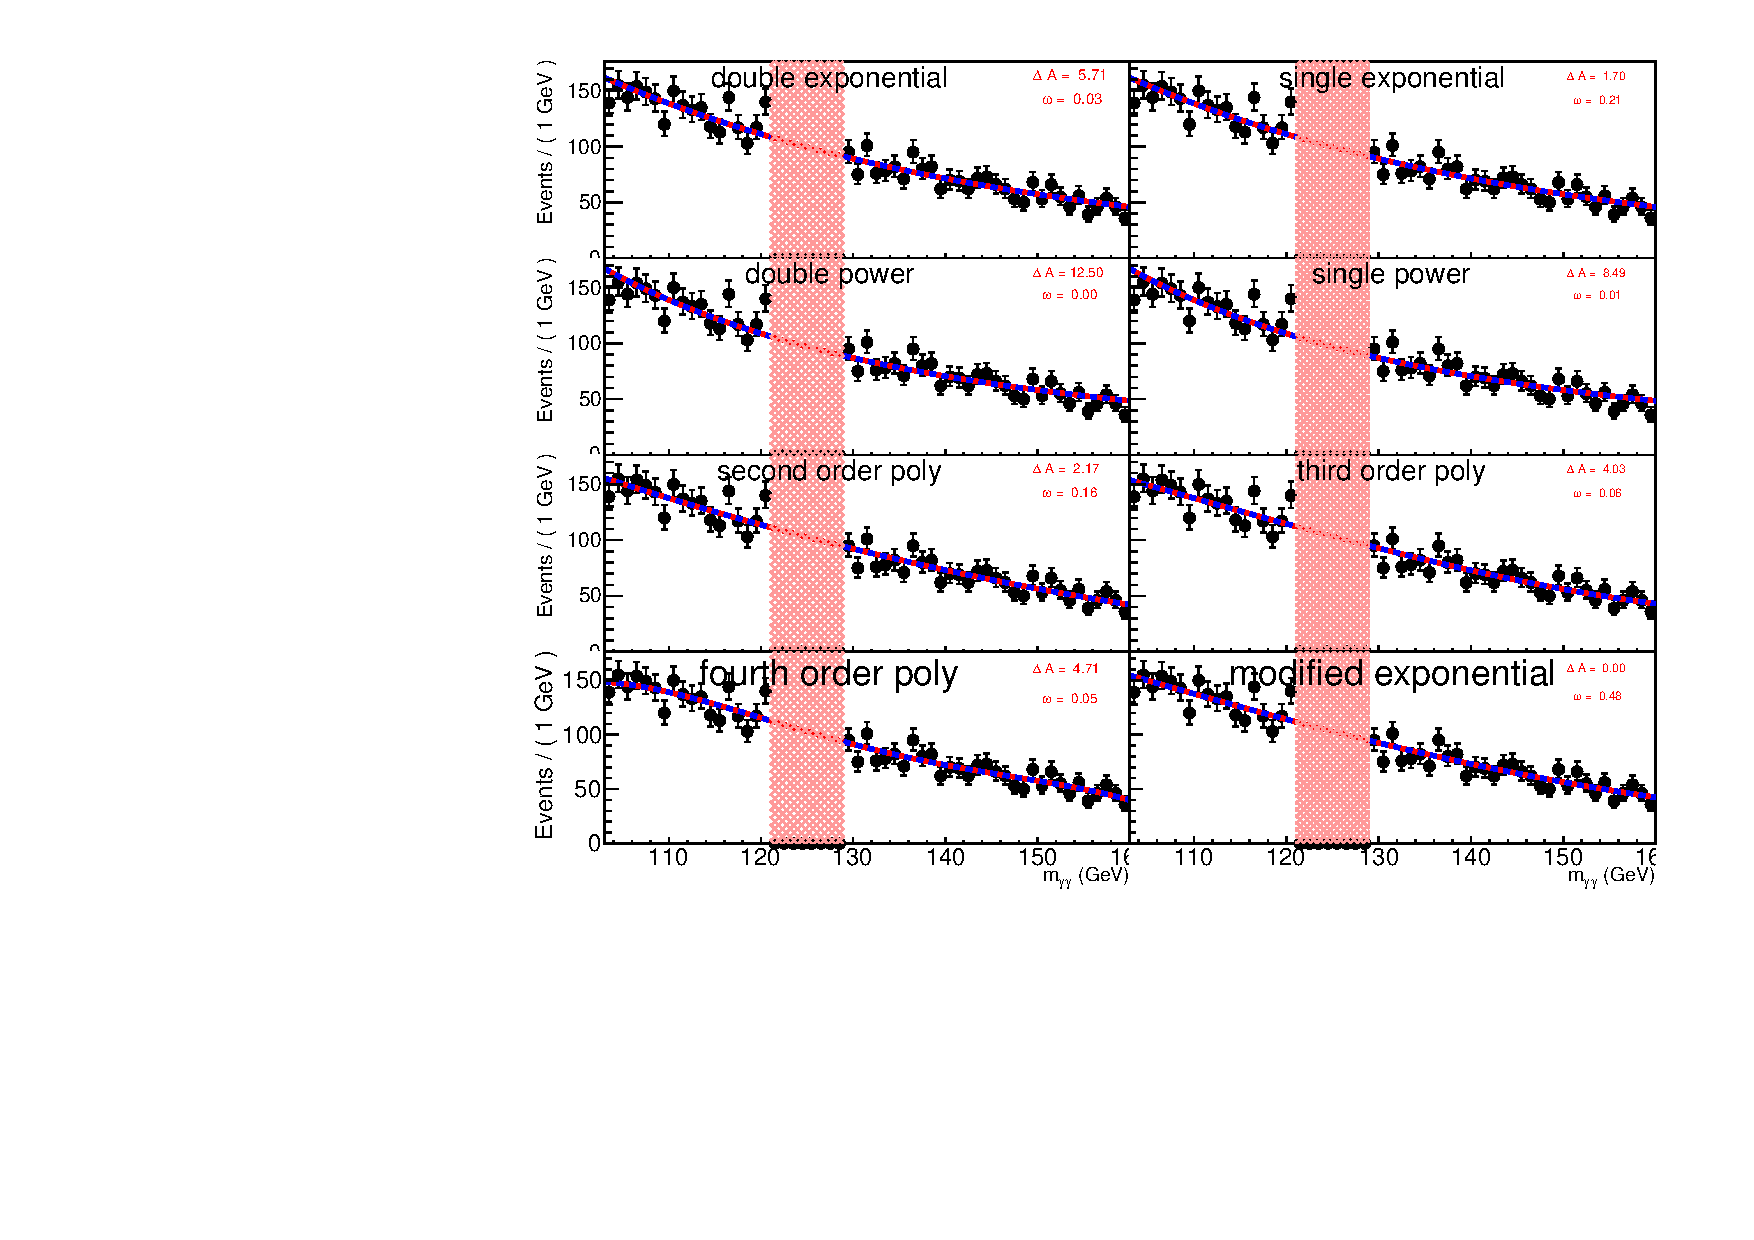
\includegraphics[width=0.6\textwidth]{hgg/highres/150_0d000.pdf} 
\caption{sideband fits for the search region: HighRes, 150 $<$ $M_R$
  $<$ 250\GeV, $R^2 > 0$} 
\label{fig:AICresults2} 
\end{center} 
\end{figure}

\begin{table*}[h] 
\begin{center} 
\topcaption{AIC results summary for the search region: HighRes, 150
  $<$ $M_R$ $<$ 250\GeV ,$R^2 > 0$.} 
\begin{tabular}{|c|c|ccc|c|} 
\hline function & \#P & $\Delta AIC$ & $\omega$ & $\omega_{max}/\omega$ & status \\ \hline 
\rowcolor[rgb]{0.31,0.78,0.47}  
modExp &  2 &  0.000 &  0.484 &  1.000 &  1,  2 \\ 
\rowcolor[rgb]{0.31,0.78,0.47}  
singleExp &  1 &  1.704 &  0.206 &  2.344 &  0,  3 \\ 
\rowcolor[rgb]{0.31,0.78,0.47}  
poly2 &  3 &  2.173 &  0.163 &  2.964 &  0,  3 \\ 
\rowcolor[rgb]{1.0,0.41,0.38}  
poly3 &  4 &  4.028 &  0.065 &  7.492 &  1,  2 \\ 
\rowcolor[rgb]{1.0,0.41,0.38}  
poly4 &  5 &  4.714 &  0.046 & 10.560 &  0,  3 \\ 
\rowcolor[rgb]{1.0,0.41,0.38}  
doubleExp &  3 &  5.708 &  0.028 & 17.359 &  1,  2 \\ 
\rowcolor[rgb]{1.0,0.41,0.38}  
singlePow &  1 &  8.492 &  0.007 & 69.817 &  0,  3 \\ 
\rowcolor[rgb]{1.0,0.41,0.38}  
doublePow &  3 & 12.496 &  0.001 & 517.007 &  0,  3 \\ 
\hline 
\end{tabular} 
\label{tab:AICresults2} 
\end{center} 
\end{table*} 

\begin{figure}[h] 
\begin{center} 
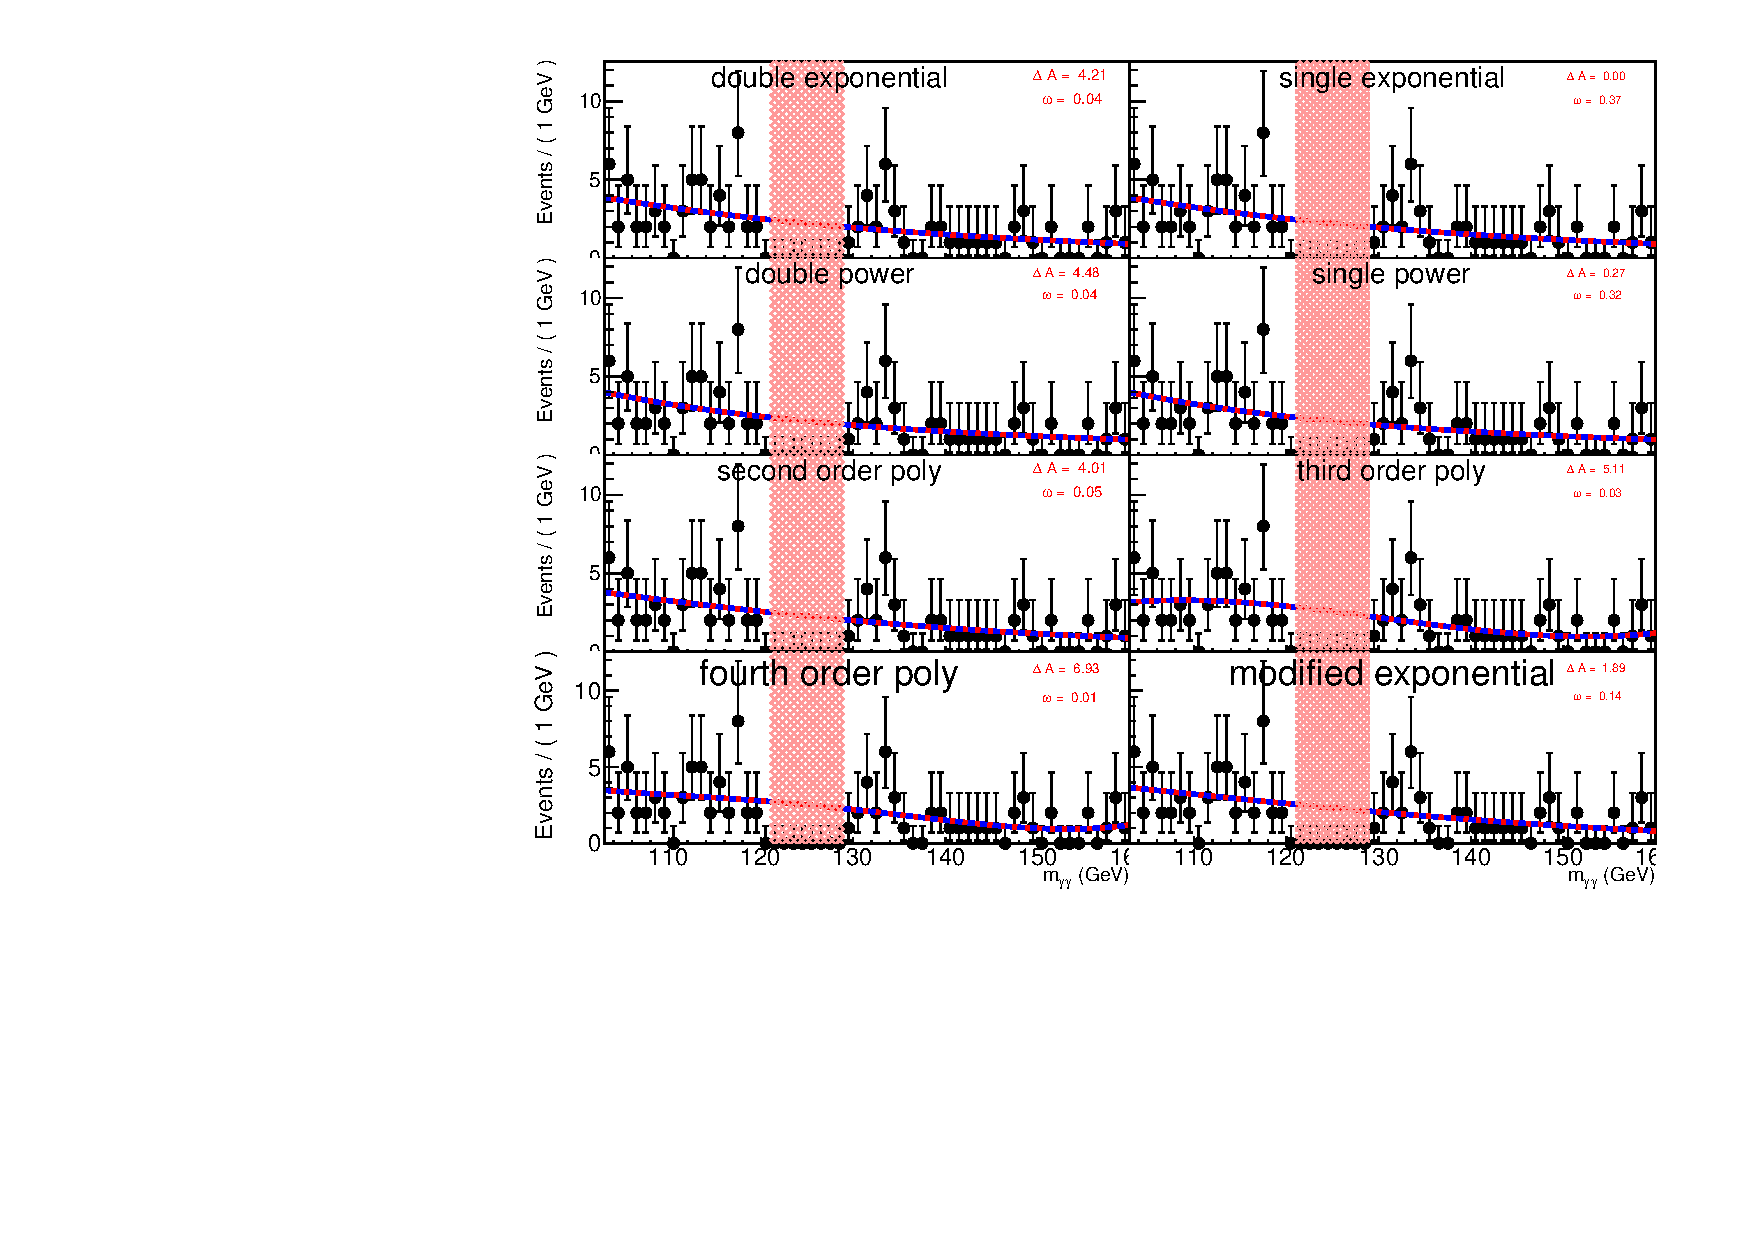
\includegraphics[width=0.6\textwidth]{hgg/lowres/150_0d175.pdf} 
\caption{Sideband fits for the search region: LowRes, 150 $<$ $M_R$
  $<$ 250\GeV, $R^2 > 0.175$.} 
\label{fig:AICresults3} 
\end{center} 
\end{figure} 

\begin{table*}[h] 
\begin{center} 
\topcaption{AIC results summary for the search region: LowRes, LowRes,
  150 $< M_R <$ 250\GeV, $R^2 > 0.175$ } 
\begin{tabular}{|c|c|ccc|c|} 
\hline function & \#P & $\Delta AIC$ & $\omega$ & $\omega_{max}/\omega$ & status \\ \hline 
\rowcolor[rgb]{0.31,0.78,0.47}  
singleExp &  1 &  0.000 &  0.529 &  1.000 &  0,  3 \\ 
\rowcolor[rgb]{0.31,0.78,0.47}  
modExp &  2 &  1.883 &  0.206 &  2.564 &  1,  2 \\ 
\rowcolor[rgb]{1.0,0.41,0.38}  
doubleExp &  3 &  3.646 &  0.085 &  6.191 &  0,  3 \\ 
\rowcolor[rgb]{1.0,0.41,0.38}  
singlePow &  1 &  3.698 &  0.083 &  6.353 &  0,  3 \\ 
\rowcolor[rgb]{1.0,0.41,0.38}  
poly2 &  3 &  4.925 &  0.045 & 11.736 &  0,  3 \\ 
\rowcolor[rgb]{1.0,0.41,0.38}  
poly3 &  4 &  5.892 &  0.028 & 19.029 &  0,  3 \\ 
\rowcolor[rgb]{1.0,0.41,0.38}  
poly4 &  5 &  7.657 &  0.012 & 45.992 &  0,  3 \\ 
\rowcolor[rgb]{1.0,0.41,0.38}  
doublePow &  3 &  7.703 &  0.011 & 47.065 &  1,  2 \\ 
\hline 
\end{tabular} 
\label{tab:AICresults3} 
\end{center} 
\end{table*} 

\begin{figure}[h] 
\begin{center} 
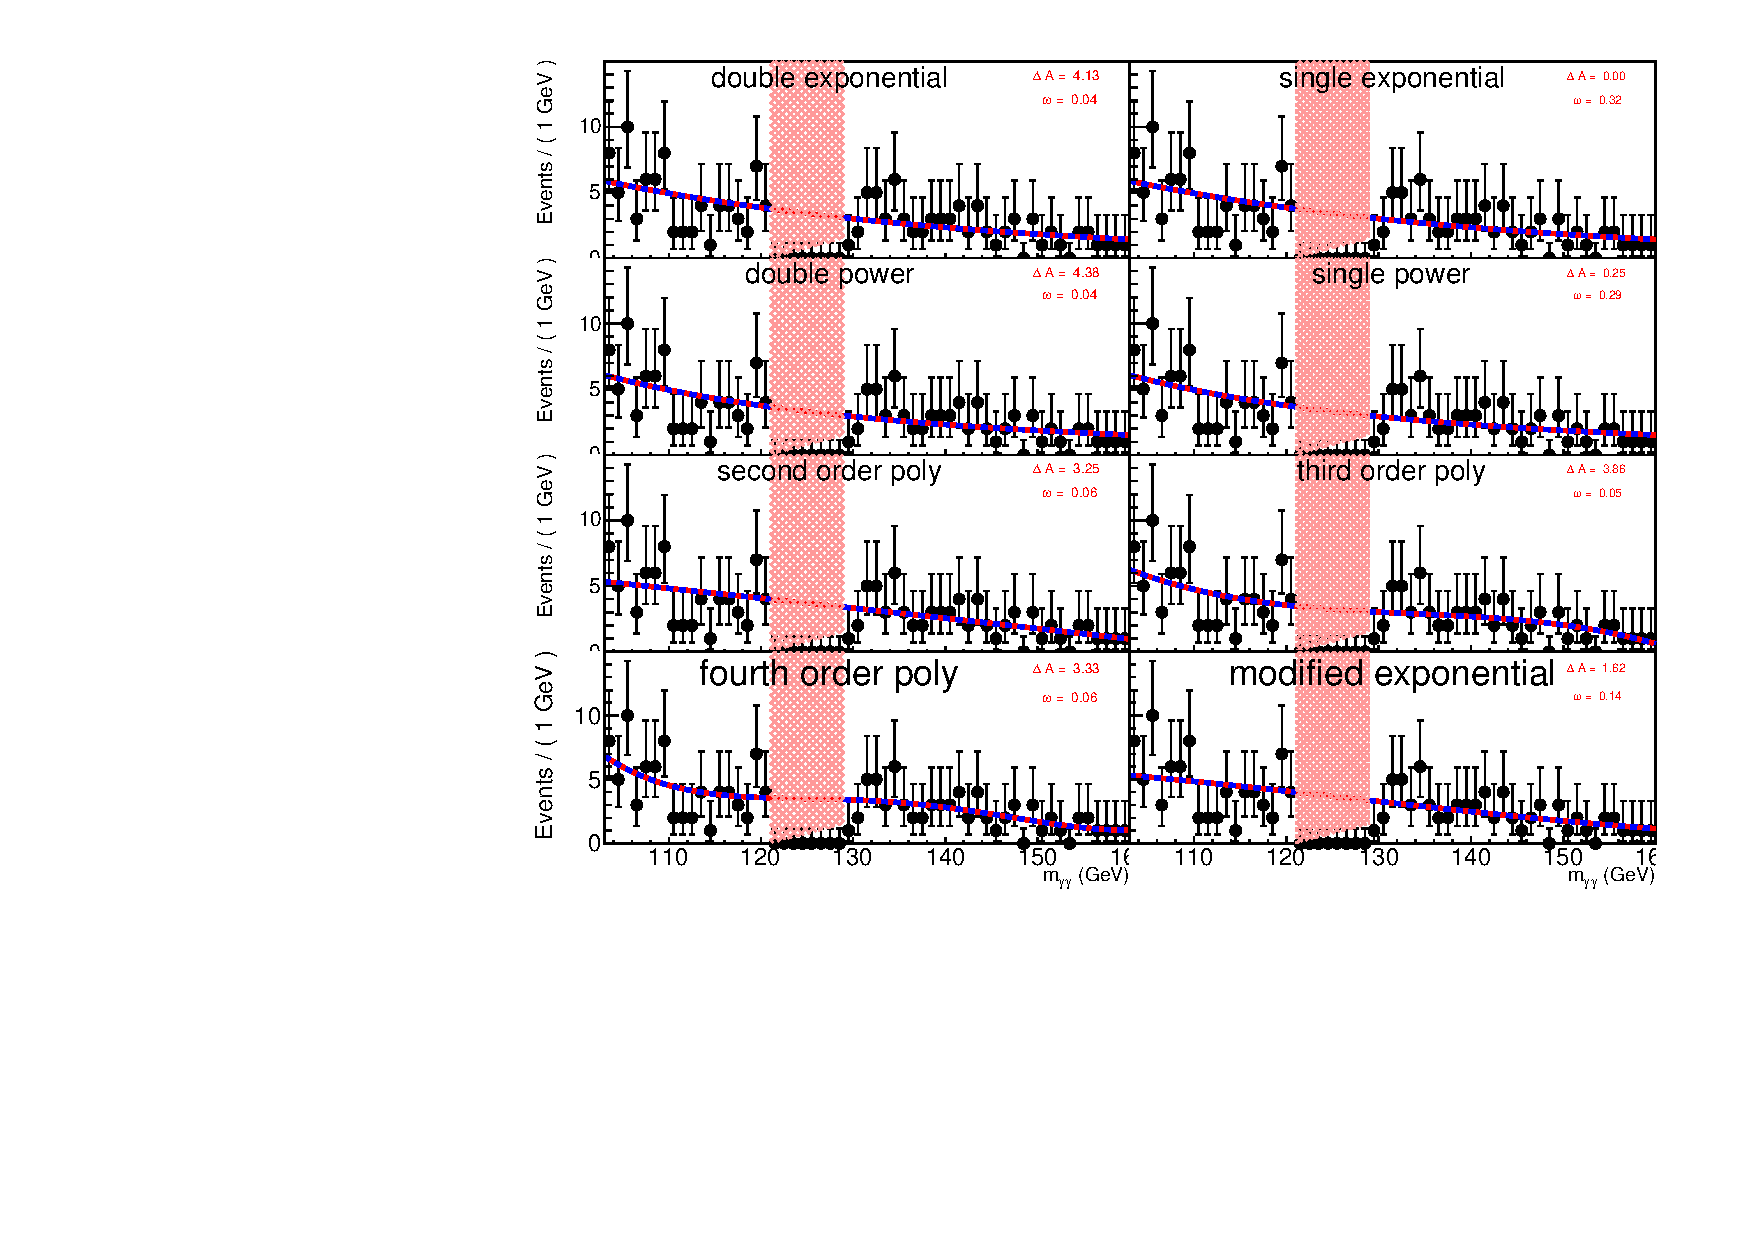
\includegraphics[width=0.6\textwidth]{hgg/hzbb/150_0d00.pdf} 
\caption{Sideband fits for the search region:
  H($\gamma\gamma$)-H/Z(bb), $M_R > 150$\GeV , $R^2 > 0$.} 
\label{fig:AICresults4} 
\end{center} 
\end{figure} 

\begin{table*}[h] 
\begin{center} 
\topcaption{AIC results summary for the search region:
  H($\gamma\gamma$)-H/Z(bb), $M_R > 150$\GeV, $R^2 > 0$.} 
\begin{tabular}{|c|c|ccc|c|} 
\hline function & \#P & $\Delta AIC$ & $\omega$ & $\omega_{max}/\omega$ & status \\ \hline 
\rowcolor[rgb]{0.31,0.78,0.47}  
singleExp &  1 &  0.000 &  0.323 &  1.000 &  0,  3 \\ 
\rowcolor[rgb]{0.31,0.78,0.47}  
singlePow &  1 &  0.247 &  0.285 &  1.131 &  0,  3 \\ 
\rowcolor[rgb]{0.31,0.78,0.47}  
modExp &  2 &  1.619 &  0.144 &  2.247 &  1,  2 \\ 
\rowcolor[rgb]{1.0,0.41,0.38}  
poly2 &  3 &  3.252 &  0.063 &  5.083 &  0,  3 \\ 
\rowcolor[rgb]{1.0,0.41,0.38}  
poly4 &  5 &  3.334 &  0.061 &  5.297 &  0,  3 \\ 
\rowcolor[rgb]{1.0,0.41,0.38}  
poly3 &  4 &  3.858 &  0.047 &  6.881 &  0,  3 \\ 
\rowcolor[rgb]{1.0,0.41,0.38}  
doubleExp &  3 &  4.134 &  0.041 &  7.901 &  0,  3 \\ 
\rowcolor[rgb]{1.0,0.41,0.38}  
doublePow &  3 &  4.382 &  0.036 &  8.946 &  0,  3 \\ 
\hline 
\end{tabular} 
\label{tab:AICresults4} 
\end{center} 
\end{table*} 
\clearpage
The second step is the bias test, where only functions that passed the
AIC test are considered. The bias test quantifies the error on the
measured signal made when
performing a signal-plus-background fit to the entire
$m_{\gamma\gamma}$ region in the final stage of the analysis. By
requiring the selected function to have a small bias relative to any of
the functions passing the AIC test, the error on the measured signal
strength is reduced. In this analysis, the bias is defined relative to
the fit uncertainty on the signal, i.e.
\begin{equation}
\label{eq:bias}
\delta s = \frac{\hat{N}_{s}-N_{s}}{\sigma_{N_{s}}},
\end{equation}
where $\hat{N}_{s}$ is the fitted signal, $N_{s}$ is the
actual value of the signal, and $\sigma_{N_{s}}$ is the
uncertainty on $\hat{N}_{s}$. The bias estimation is obtained by
carrying a large number of pseudo-experiments (toys), each function
passing the AIC test will be treated as the parent function from where
the data was drawn, then several (10,000) toy datasets will be drawn from
it containing the same amount of event as in the real dataset. For
each toy dataset a know number of signal event will be injected ($N_{s}$) and a signal-plus-background fit will be carried out and
the bias will be calculated. After this procedure is done, the
resulting bias distribution will be fitted with a double-sided
crystal ball function, where the most probable value after the fit is
taken as an estimate of the bias. Figure~\ref{fig:biasExample} shows
the resulting bias distribution and fit for two different
cases. The studies carried out indicate that the most stringent test
occurs when the number of injected signal events is small ( signal to
background ratio or S/B equal to zero) and therefore the results shown
here correspond to that case. Table~\ref{table:biasExample} shows the bias estimates for one of
the search regions, where you can see the relative biases for all
possible function passing the AIC test. Finally, the function with the
least numer of free parameters and having a relative bias smaller than
30\% -- which yield only an additional error of 5\% -- is selected as
the background model. The final selection for all the signal regions
is shown in Table~\ref{tab:modelSelectionSummary_15ifb}.
\begin{figure}[h]
\begin{center}
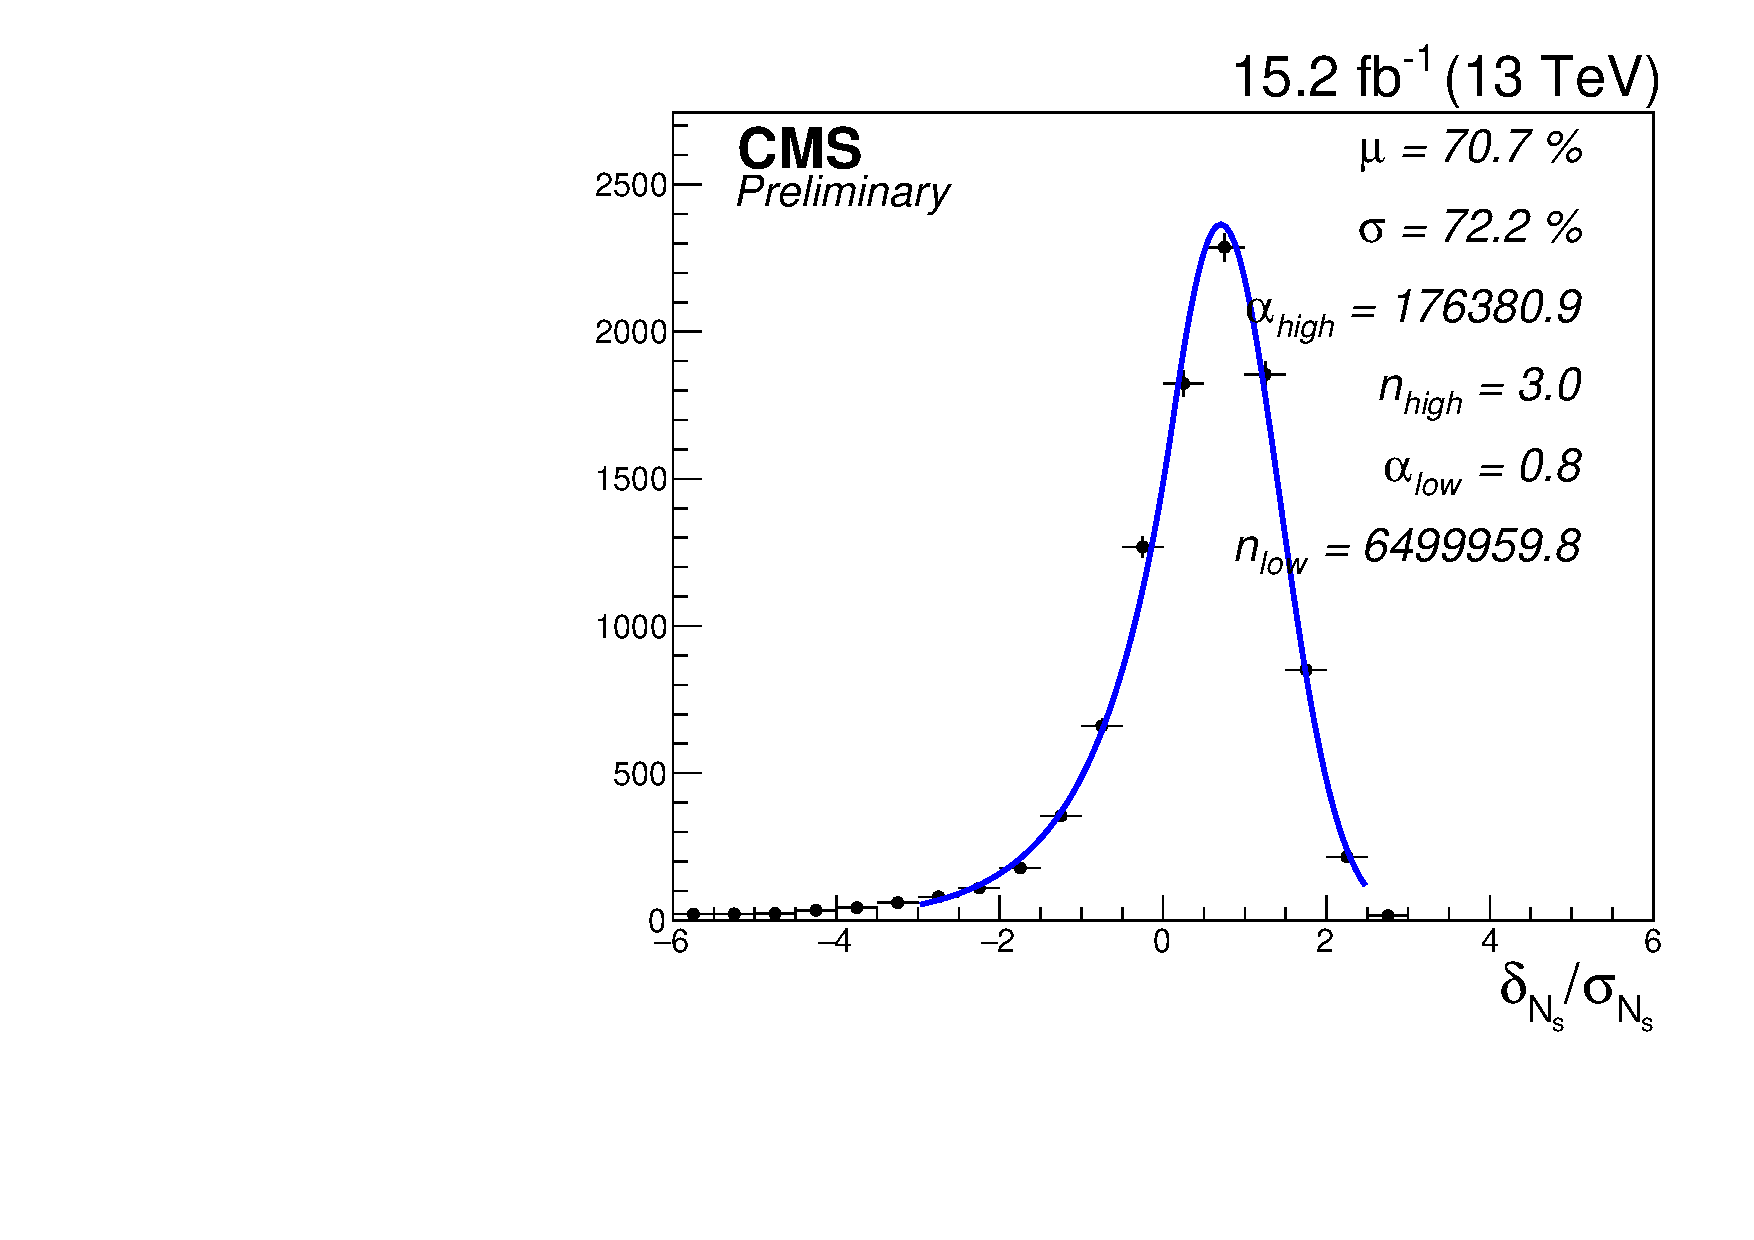
\includegraphics[width=0.45\textwidth]{hgg/doubleTailCrystalBall_biasFits_poly3_singleExp.pdf}
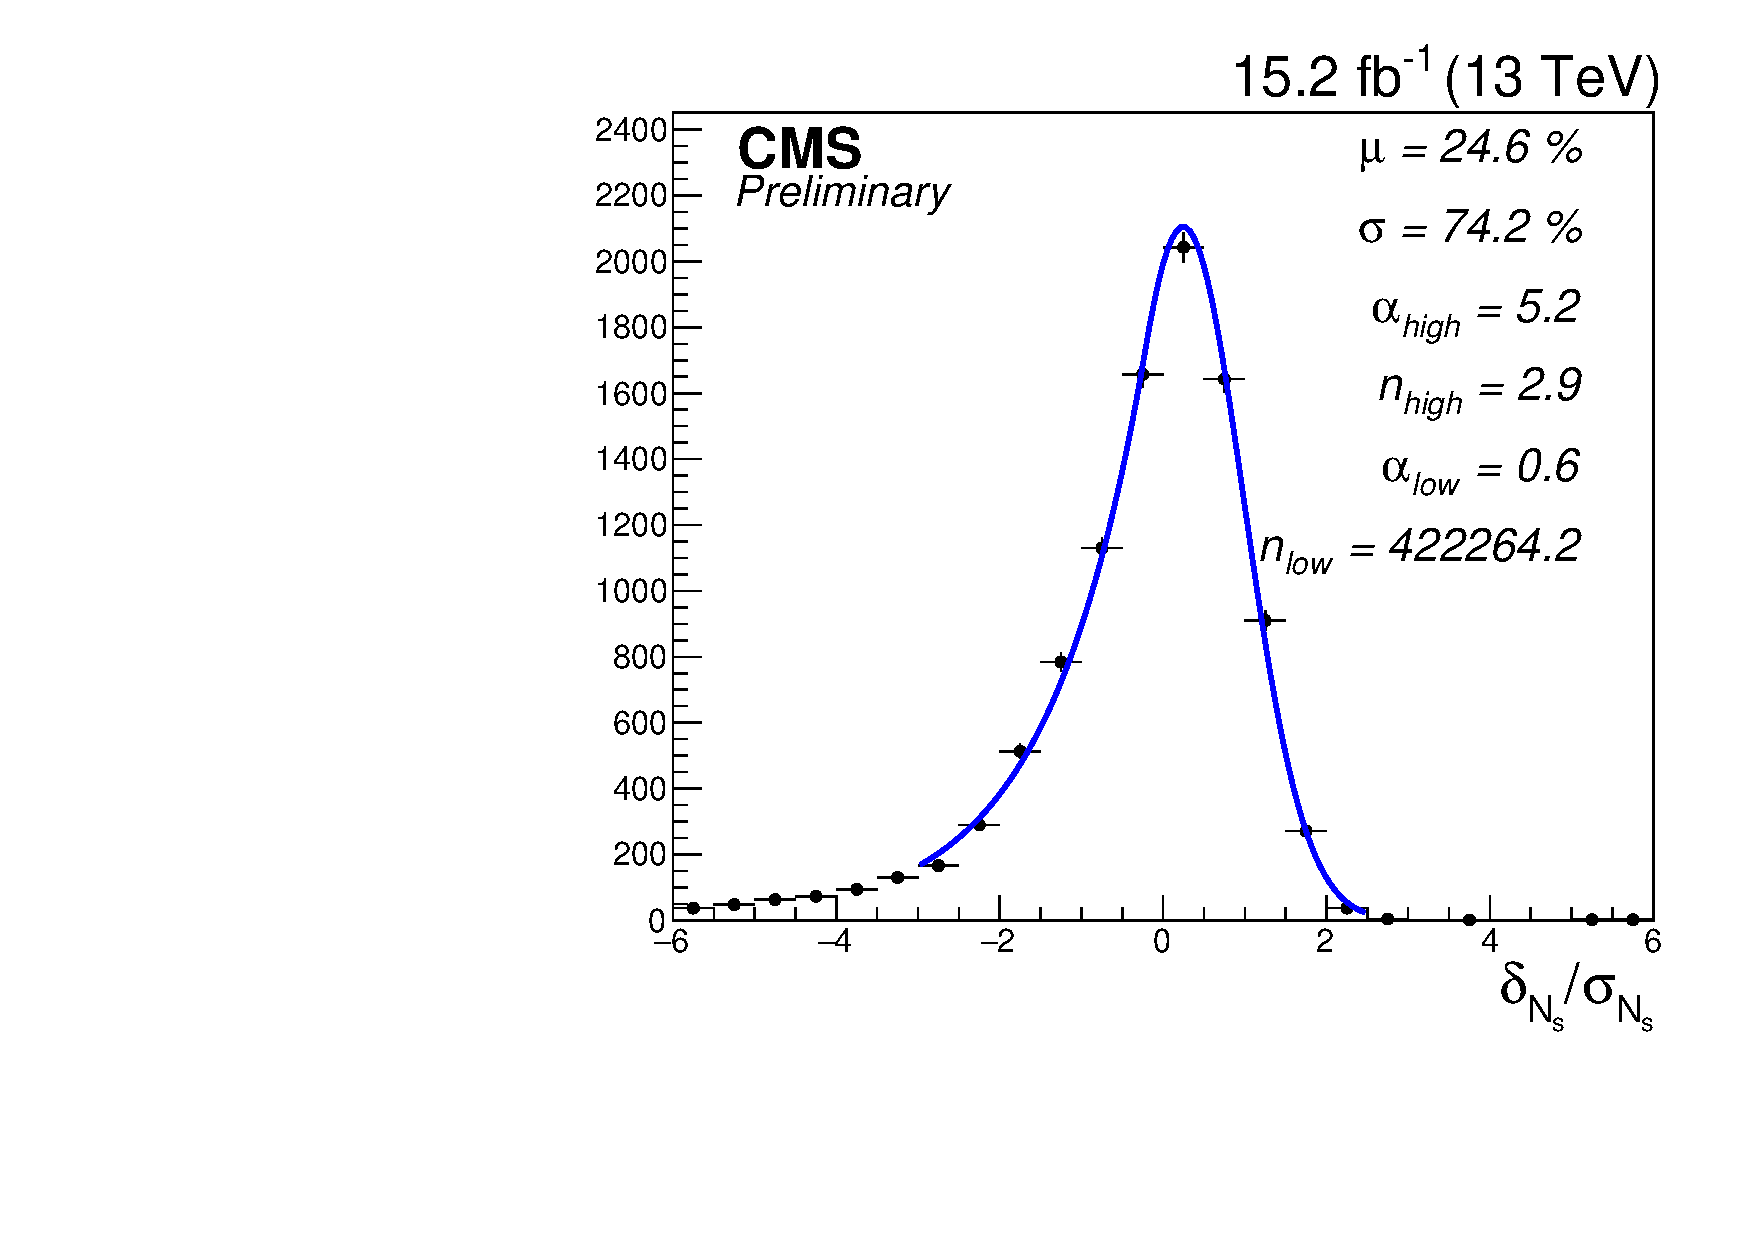
\includegraphics[width=0.45\textwidth]{hgg/doubleTailCrystalBall_biasFits_poly3_poly3.pdf}
\caption{Examples of the bias distribution for bin0 (HighPt, $M_R>600, R^2>0.025$). Left: $f_{1}$ (assumed parent function) = poly3, $f_{2}$ (tested function) = singleExp; right: $f_{1}$ = poly3, $f_{2}$ =  poly3. From the left plot we can see that singleExp does not pass the bias test since it has large bias to fit poly3.  }
\label{fig:biasExample}
\end{center}
\end{figure}

\begin{table}[h]
\begin{center}
\topcaption{Examples of the bias estimate for diffrent function pairs
  passing the AIC test for bin0 (HighPt, $M_R>600, R^2>0.025$). 
Functiosn in the first column are the assumed parent functions
($f_{1}$), while functions 
in the first row are the ones being tested ($f_{2}$). In the first row,
the numbers in brackets are the AIC weights. }
\begin{tabular}{|c|c|c|c|c|}
\hline
-- & singlePow(0.247) & singleExp(0.232) & poly3(0.183) & poly2(0.177) \\
\hline
singlePow & (21.3$\pm$ 1.0)\% & (19.3$\pm$ 1.0)\% & (17.8$\pm$ 1.0)\% & (18.5$\pm$ 1.4)\% \\
singleExp & (22.9$\pm$ 2.0)\% & (18.3$\pm$ 1.0)\% & (7.9$\pm$ 1.3)\% & (18.7$\pm$ 2.0)\% \\
poly3 & (69.9$\pm$ 1.5)\% & (70.7$\pm$ 0.9)\% & (24.6$\pm$ 1.3)\% & (33.5$\pm$ 1.0)\% \\
poly2 & (60.6$\pm$ 0.9)\% & (62.6$\pm$ 0.9)\% & (15.7$\pm$ 1.9)\% & (17.4$\pm$ 1.4)\% \\
\hline
\end{tabular}
\label{table:biasExample}
\end{center}
\end{table}
\begin{table*}[h]
\begin{center}
\topcaption{List of the selected background functions for different search
  regions.}
\tiny
\begin{tabular}{|c|c|cccc|c|cc|}
\hline
Bin & Category & LowMR & HighMR & LowRsq & HighRsq & Function & AIC weight & Max bias / $\sigma_{\mathrm{stat}}$ \\ 
\hline
0 & highpt & 600 & 10000 & 0.025 & 10.000 & poly3 & 0.183 & 24.6\%\\
1 & highpt & 150 & 600 & 0.130 & 10.000 & singleExp & 0.356 & 17.7\%\\
2 & highpt & 1250 & 10000 & 0.000 & 0.025 & singleExp & 0.359 & 16.4\%\\
3 & highpt & 150 & 450 & 0.000 & 0.130 & -- & -- & --\%\\
4 & highpt & 450 & 600 & 0.000 & 0.035 & poly2 & 0.324 & -24.2\%\\
5 & highpt & 450 & 600 & 0.035 & 0.130 & singleExp & 0.348 & 16.1\%\\
6 & highpt & 600 & 1250 & 0.000 & 0.015 & singleExp & 0.295 & -3.6\%\\
7 & highpt & 600 & 1250 & 0.015 & 0.025 & singleExp & 0.344 & 14.8\%\\
\hline
8 & hzbb & 150 & 2000 & 0.00 & 10.000 & singleExp & 0.323 & 4.5\%\\ 
\hline
9 & highres & 150 & 250 & 0.000 & 0.175 & -- & -- & --\%\\
10 & highres & 150 & 250 & 0.175 & 10.000 & poly2 & 0.132 & 16.9\%\\
11 & highres & 250 & 10000 & 0.05 & 10.000 & singlePow & 0.237 & -19.1\%\\
12 & highres & 250 & 600 & 0.000 & 0.05 & singlePow & 0.118 & 25.7\%\\
13 & highres & 600 & 10000 & 0.000 & 0.05 & singleExp & 0.256 & -3.4\%\\
\hline
14 & lowres & 150 & 250 & 0.000 & 0.175 & singleExp & 0.529 & -3.4\%\\
15 & lowres & 150 & 250 & 0.175 & 10.000 & singleExp & 0.365 & 7.9\%\\
16 & lowres & 250 & 10000 & 0.05 & 10.000 & singleExp & 0.358 & -13.9\%\\
17 & lowres &  250 & 600 & 0.000 & 0.05 & --  & --  &  --\%\\
18 & lowres & 600 & 10000 & 0.000 & 0.05 & singleExp & 0.364 & -9.0\%\\
\hline
\end{tabular}
\label{tab:modelSelectionSummary_15ifb}
\end{center}
\end{table*}
\section{Systematic Uncertainties}\label{sec:systematics}
The dominant systematic uncertainty is the uncertainty on the prediction of the 
non-resonant background shape and normalization. These are propagated by
profiling the overall normalization and the shape parameters of the non-resonant
background functional form.

Sub-dominant systematic uncertainties on the SM Higgs background are propagated through
log-normal nuisance parameters, and take into account both theoretical and instrumental
effects. The effects considered include missing higher order corrections, 
parton distribution functions, trigger and selection efficiencies, jet energy scale uncertainties, 
b-tagging efficiencies, and the uncertainty on the integrated luminosity. The typical size of these 
effects on the expected limit is summarized in Table~\ref{tab:SignalSystematics}.

The systematic uncertainty on the photon energy scale is implemented as a nuisance parameter
that shifts the Higgs peak position, and is Gaussian constrained in the fit to lie within $1\%$ of the nominal 
Higgs mass peak predicted by the Monte Carlo simulation. There is also a systematic uncertainty 
on the shape of the $\sigma_{\mathrm{M}}/\mathrm{M}$ distribution, which allows for migration of 
SM Higgs background and signal events between the HighRes and the LowRes categories.

\begin{table}[!ht]
\begin{center}
\caption{Summary of systematic uncertainties and their size.}
\label{tab:SignalSystematics}
\begin{tabular}{|c|c|}
\hline
Uncertainty Source & Size \\
\hline
Luminosity                                 & 5.7\% \\
PDFs and QCD Scale Variations              & 15-30\%\\
Trigger and selection efficiency            & 3\% \\
Jet energy scale                           & 1-5\% \\
Photon Energy Scale                        & 1\% \\
B-tagging efficiency                       & 4\% \\
$\sigma_{\mathrm{M}}/\mathrm{M}$ categorization & $4\%$ \\
\hline
\end{tabular}
\end{center}
\end{table}



\section{Results and Interpretations}
\label{sec:results}

The fit results for all search regions using the combination of the 2015 dataset ($2.3~\mathrm{fb}^{-1}$)
and the 2016 dataset ($12.9~\mathrm{fb}^{-1}$) are shown below.
Figures~\ref{fig:UnblindedResultsHighPt1},~\ref{fig:UnblindedResultsHighPt2},~and~\ref{fig:UnblindedResultsHighPt3}
show the results for the HighPt event category. 
The results for the H($\gamma\gamma$)-H/Z(bb) category are shown in Figure~\ref{fig:UnblindedResultsHZbb}.
Finally, the results for the HighRes and LowRes categories are shown in 
Figures~\ref{fig:UnblindedResultsBin9}~to~\ref{fig:UnblindedResultsBin13}.

\begin{figure}[ht!]
\centering
HighPt Category: $M_{R}>600$\GeV, $R^{2}>0.025$\\
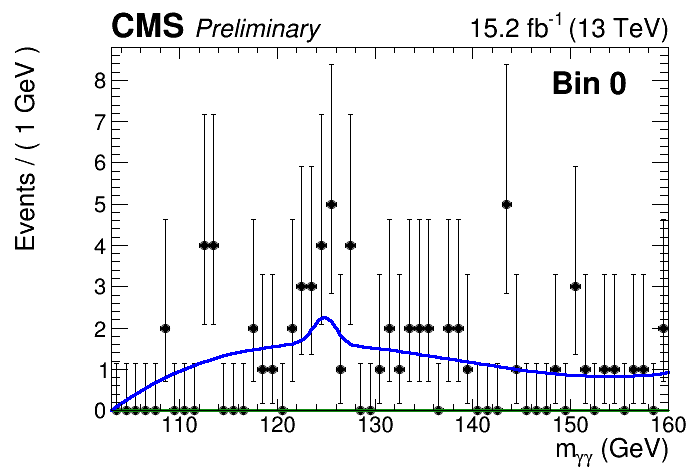
\includegraphics[width=0.45\textwidth, angle=0.]{figs/unblindedResults2p3Plus12p9/bin0_fit_b.png}
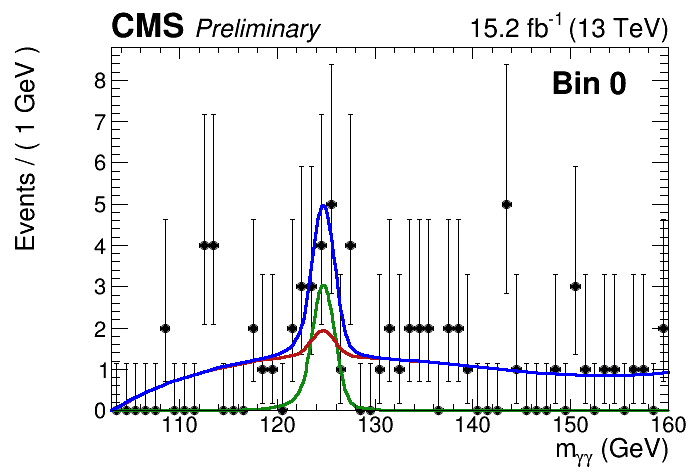
\includegraphics[width=0.45\textwidth, angle=0.]{figs/unblindedResults2p3Plus12p9/bin0_fit_s.png}\\
HighPt Category: $150 < M_{R} < 600$\GeV, $R^{2}>0.13$\\
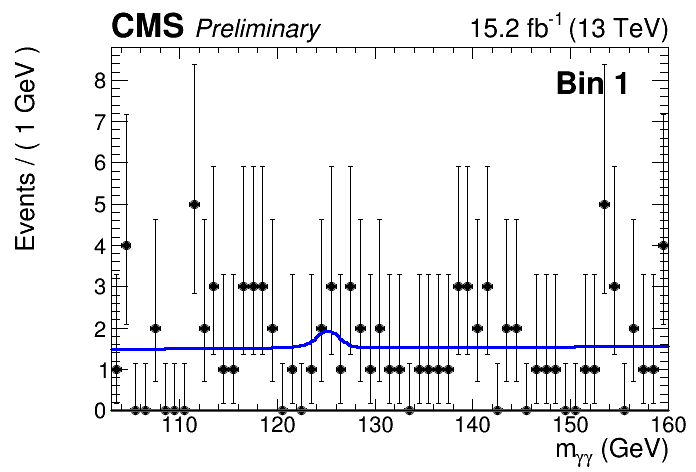
\includegraphics[width=0.45\textwidth, angle=0.]{figs/unblindedResults2p3Plus12p9/bin1_fit_b.png}
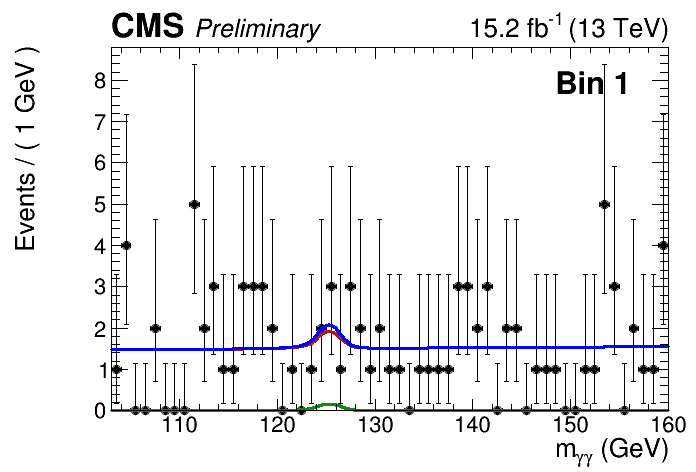
\includegraphics[width=0.45\textwidth, angle=0.]{figs/unblindedResults2p3Plus12p9/bin1_fit_s.png}\\
HighPt Category: $M_{R}>1250$\GeV, $0 < R^{2} < 0.025$\\
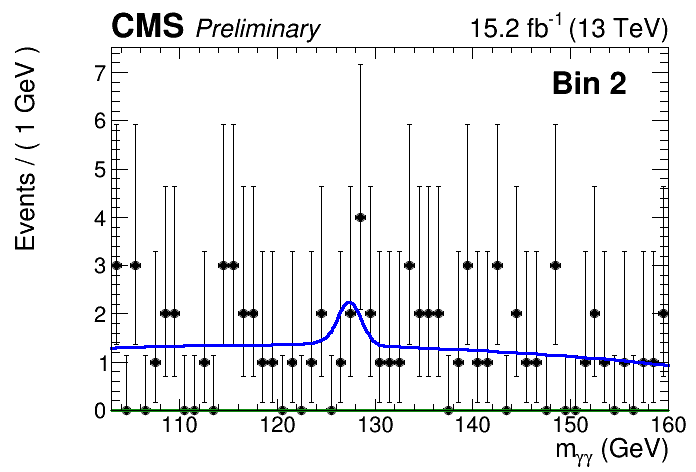
\includegraphics[width=0.45\textwidth, angle=0.]{figs/unblindedResults2p3Plus12p9/bin2_fit_b.png}
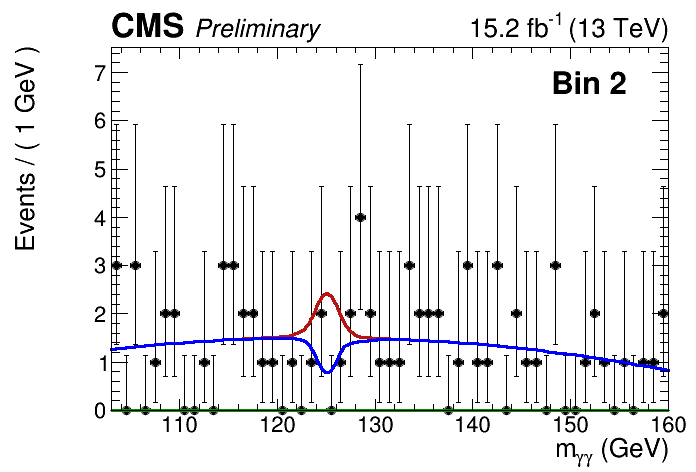
\includegraphics[width=0.45\textwidth, angle=0.]{figs/unblindedResults2p3Plus12p9/bin2_fit_s.png}\\
\caption{ The diphoton mass distribution for various search region bins in the HighPt category 
are shown along with the background-only fit (left) and the signal plus background fit (right). 
The red curve represents the background prediction; the green curve represents the signal; 
and the blue curve represents the sum of the signal and background. The definition of the search bin
is labeled above each pair of plots.
\label{fig:UnblindedResultsHighPt1}}
\end{figure}


\begin{figure}[ht!]
\centering
HighPt Category: $150 < M_{R} < 450$\GeV, $0 < R^{2} < 0.13$\\
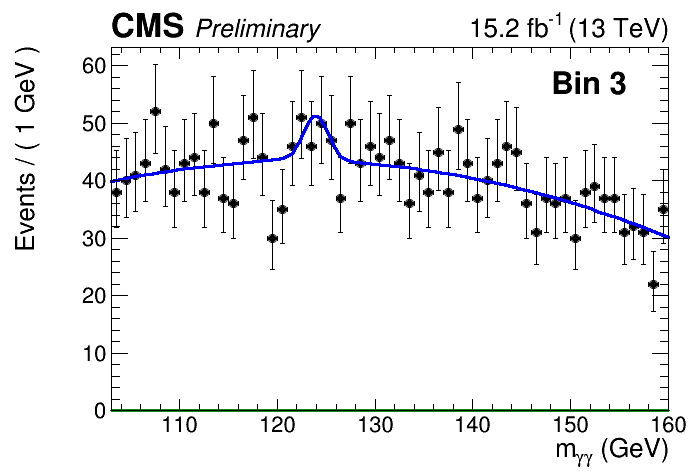
\includegraphics[width=0.45\textwidth, angle=0.]{figs/unblindedResults2p3Plus12p9/bin3_fit_b.png}
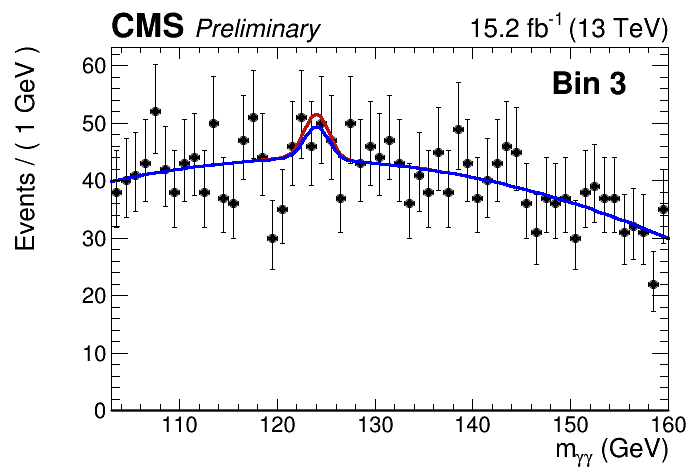
\includegraphics[width=0.45\textwidth, angle=0.]{figs/unblindedResults2p3Plus12p9/bin3_fit_s.png}\\
HighPt Category: $450 < M_{R} < 600$\GeV, $0 < R^{2} < 0.035$\\
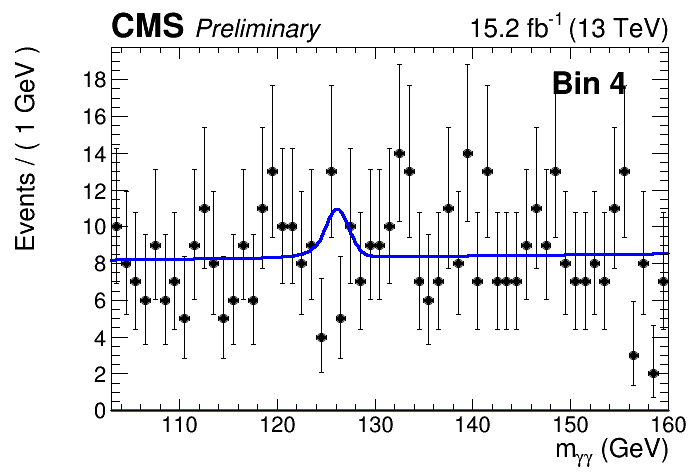
\includegraphics[width=0.45\textwidth, angle=0.]{figs/unblindedResults2p3Plus12p9/bin4_fit_b.png}
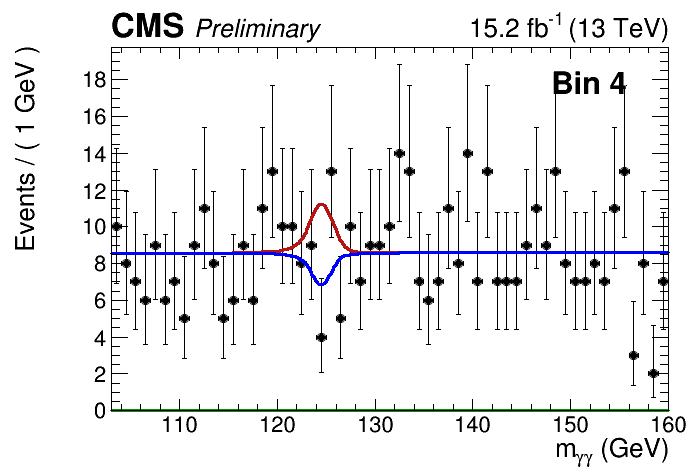
\includegraphics[width=0.45\textwidth, angle=0.]{figs/unblindedResults2p3Plus12p9/bin4_fit_s.png}\\
HighPt Category: $450 < M_{R} < 600$\GeV, $0.13 < R^{2} < 0.035$\\
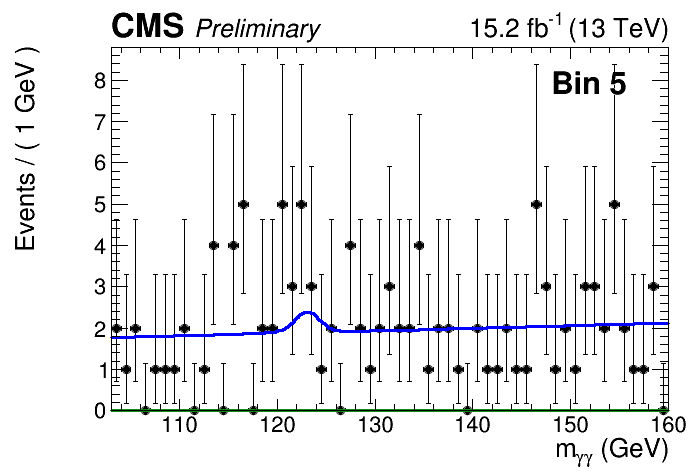
\includegraphics[width=0.45\textwidth, angle=0.]{figs/unblindedResults2p3Plus12p9/bin5_fit_b.png}
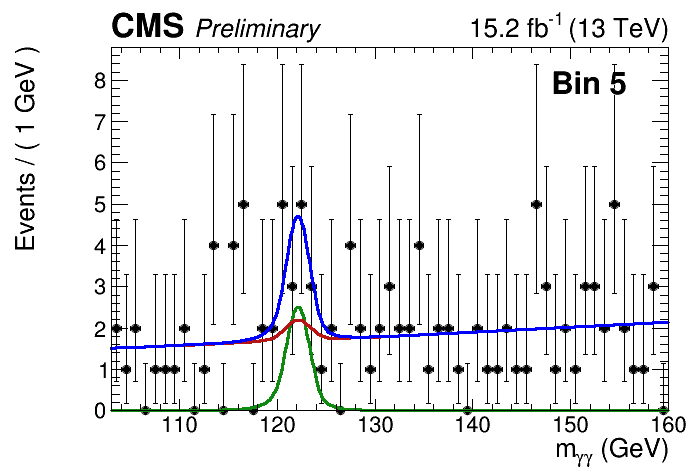
\includegraphics[width=0.45\textwidth, angle=0.]{figs/unblindedResults2p3Plus12p9/bin5_fit_s.png}\\
\caption{ The diphoton mass distribution for various search region bins in the HighPt category 
are shown along with the background-only fit (left) and the signal plus background fit (right). 
The red curve represents the background prediction; the green curve represents the signal; 
and the blue curve represents the sum of the signal and background. The definition of the bin
is labeled above each pair of plots.
\label{fig:UnblindedResultsHighPt2}}
\end{figure}


\begin{figure}[ht!]
\centering
HighPt Category: $600 < M_{R} < 1250$\GeV, $0 < R^{2} < 0.015$\\
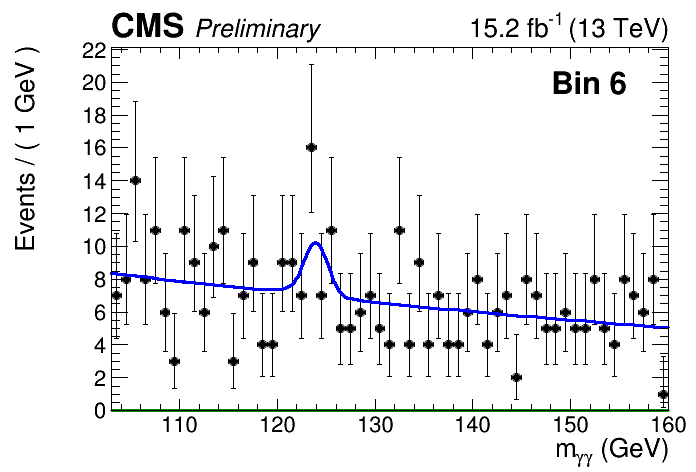
\includegraphics[width=0.45\textwidth, angle=0.]{figs/unblindedResults2p3Plus12p9/bin6_fit_b.png}
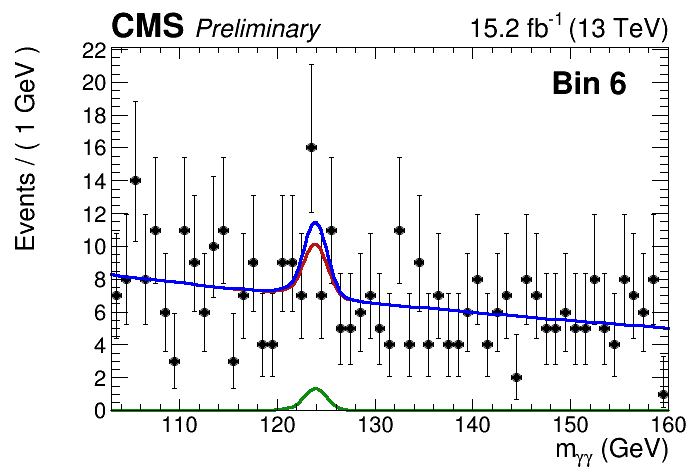
\includegraphics[width=0.45\textwidth, angle=0.]{figs/unblindedResults2p3Plus12p9/bin6_fit_s.png}\\
HighPt Category: $600 < M_{R} < 1250$\GeV, $0.015 < R^{2} < 0.025$\\
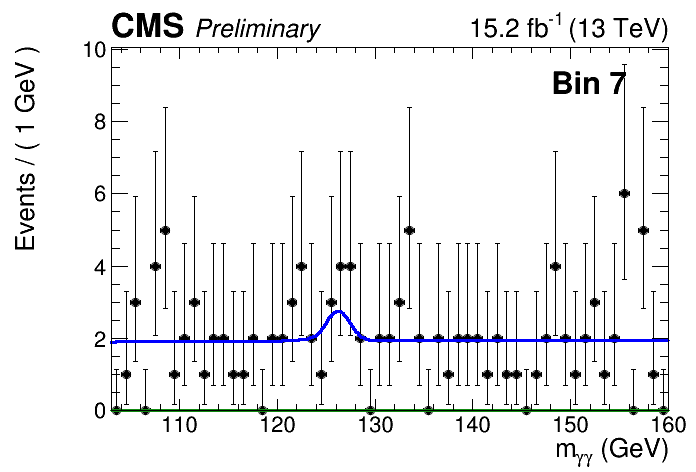
\includegraphics[width=0.45\textwidth, angle=0.]{figs/unblindedResults2p3Plus12p9/bin7_fit_b.png}
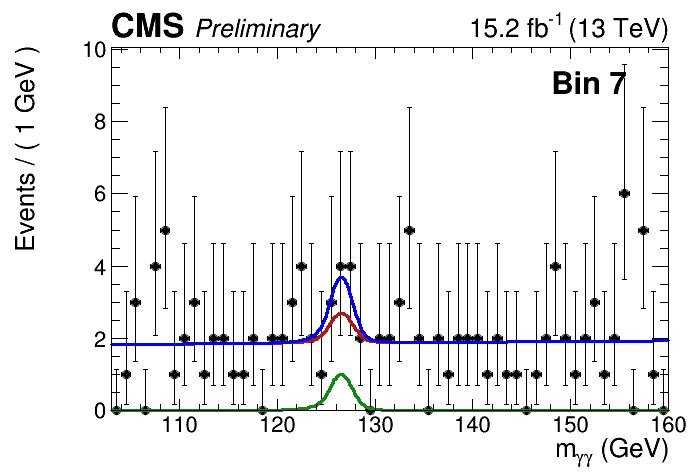
\includegraphics[width=0.45\textwidth, angle=0.]{figs/unblindedResults2p3Plus12p9/bin7_fit_s.png}\\
\caption{ The diphoton mass distribution for various search region bins in the HighPt category 
are shown along with the background-only fit (left) and the signal plus background fit (right). 
The red curve represents the background prediction; the green curve represents the signal; 
and the blue curve represents the sum of the signal and background. The definition of the bin
is labeled above each pair of plots.
\label{fig:UnblindedResultsHighPt3}}
\end{figure}


\begin{figure}[ht!]
\centering
H($\gamma\gamma$)-H/Z(bb) Category: $M_{R}>150$\GeV \\
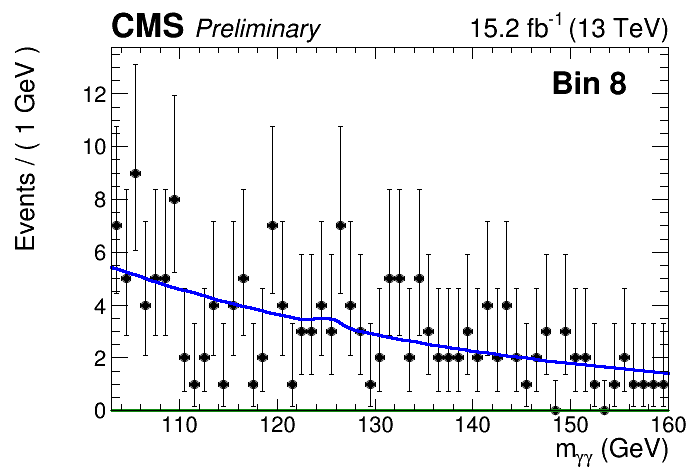
\includegraphics[width=0.45\textwidth, angle=0.]{figs/unblindedResults2p3Plus12p9/bin8_fit_b.png}
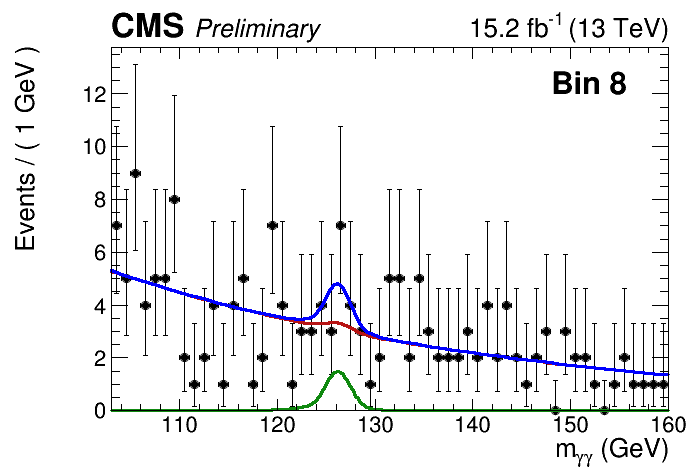
\includegraphics[width=0.45\textwidth, angle=0.]{figs/unblindedResults2p3Plus12p9/bin8_fit_s.png}\\
\caption{ The diphoton mass distribution for various search region bins in the H($\gamma\gamma$)-H/Z(bb) category 
are shown along with the background-only fit (left) and the signal plus background fit (right). 
The red curve represents the background prediction; the green curve represents the signal; 
and the blue curve represents the sum of the signal and background. The definition of the bin
is labeled above each pair of plots.
\label{fig:UnblindedResultsHZbb}}
\end{figure}


\begin{figure}[ht!]
\centering
HighRes: $150 < M_{R} < 250$\GeV, $0 < R^{2}>0.175$\\
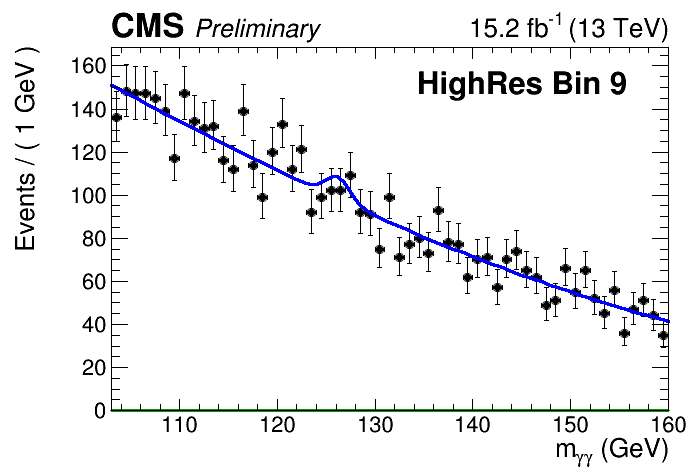
\includegraphics[width=0.45\textwidth, angle=0.]{figs/unblindedResults2p3Plus12p9/highResBin9_fit_b.png}
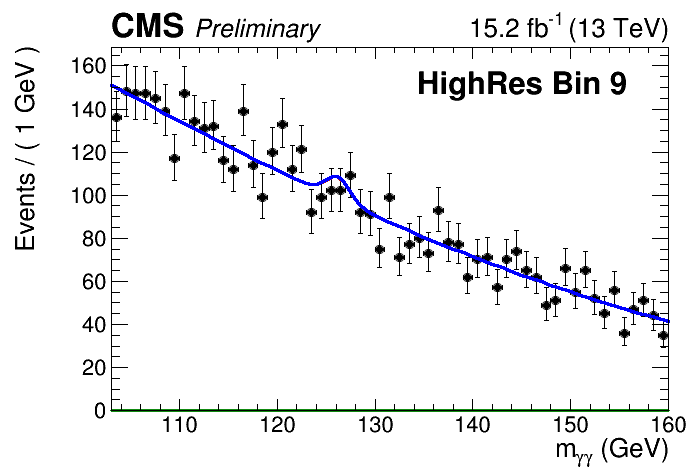
\includegraphics[width=0.45\textwidth, angle=0.]{figs/unblindedResults2p3Plus12p9/highResBin9_fit_s.png}\\
LowRes: $150 < M_{R} < 250$\GeV, $0 < R^{2}>0.175$\\
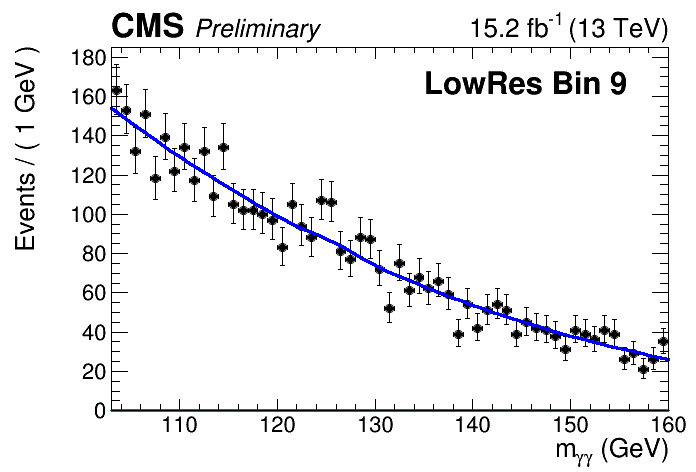
\includegraphics[width=0.45\textwidth, angle=0.]{figs/unblindedResults2p3Plus12p9/lowResBin9_fit_b.png}
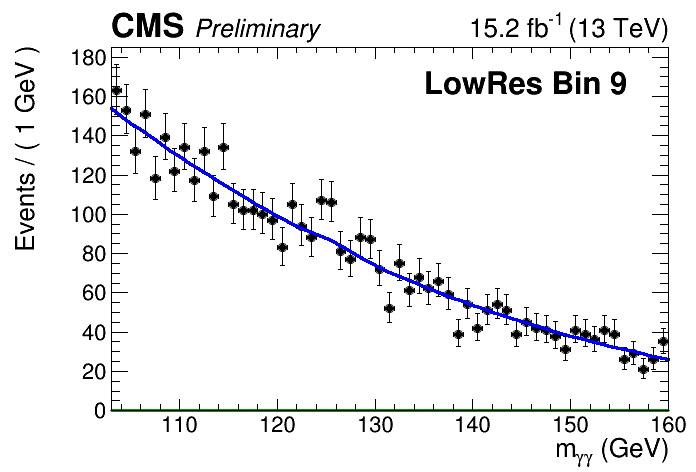
\includegraphics[width=0.45\textwidth, angle=0.]{figs/unblindedResults2p3Plus12p9/lowResBin9_fit_s.png}\\
\caption{ The diphoton mass distribution for the search region bin 9 
are shown along with the background-only fit (left) and the signal plus background fit (right).
The top row shows the HighRes category, while the bottom row shows the LowRes category.
The red curve represents the background prediction; the green curve represents the signal; 
and the blue curve represents the sum of the signal and background. The definition of the bin
is labeled above each pair of plots.
\label{fig:UnblindedResultsBin9}}
\end{figure}

\begin{figure}[ht!]
\centering
HighRes: $150 < M_{R} < 250$\GeV, $0 < R^{2}>0.175$\\
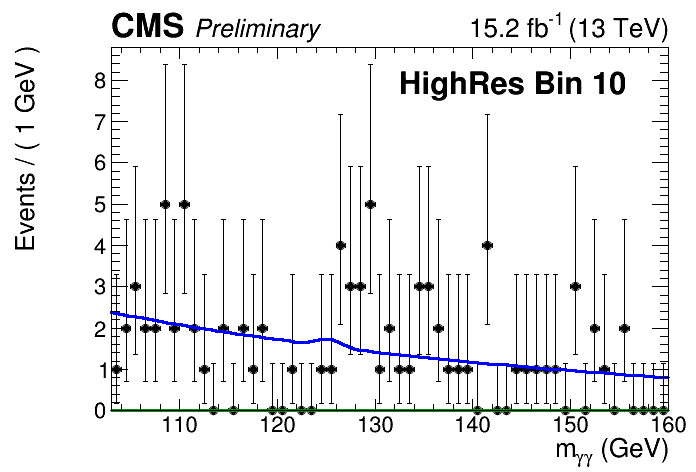
\includegraphics[width=0.45\textwidth, angle=0.]{figs/unblindedResults2p3Plus12p9/highResBin10_fit_b.png}
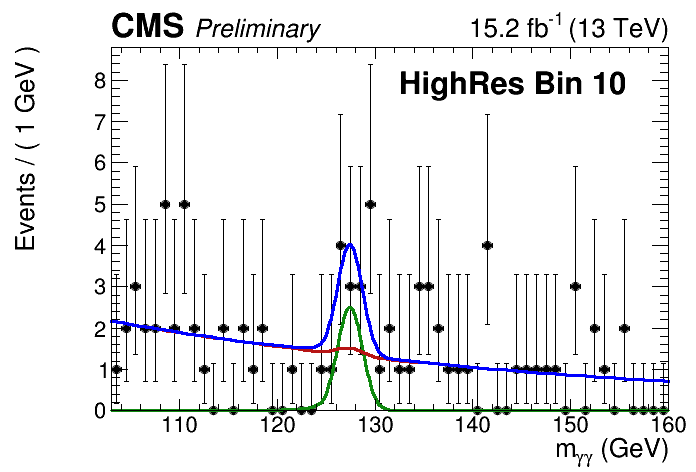
\includegraphics[width=0.45\textwidth, angle=0.]{figs/unblindedResults2p3Plus12p9/highResBin10_fit_s.png}\\
LowRes: $150 < M_{R} < 250$\GeV, $0 < R^{2}>0.175$\\
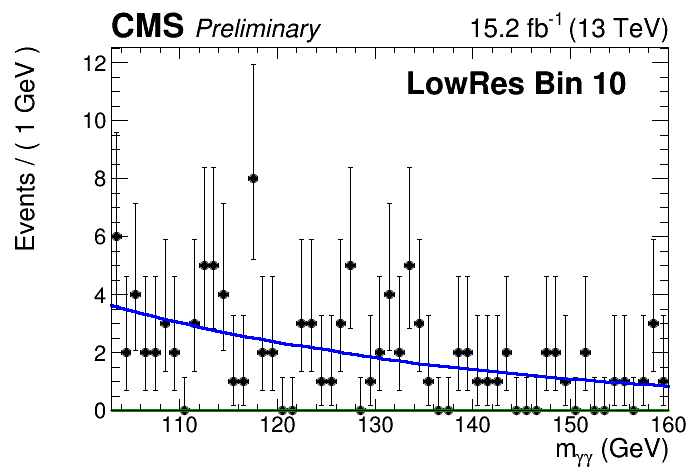
\includegraphics[width=0.45\textwidth, angle=0.]{figs/unblindedResults2p3Plus12p9/lowResBin10_fit_b.png}
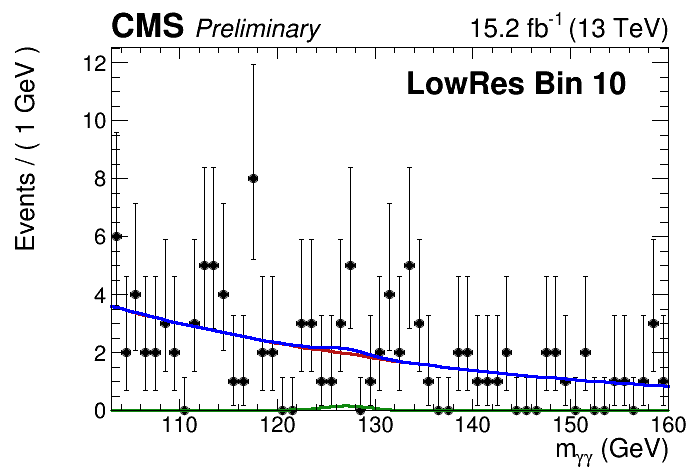
\includegraphics[width=0.45\textwidth, angle=0.]{figs/unblindedResults2p3Plus12p9/lowResBin10_fit_s.png}\\
\caption{ The diphoton mass distribution for the search region bin 10 
are shown along with the background-only fit (left) and the signal plus background fit (right).
The top row shows the HighRes category, while the bottom row shows the LowRes category.
The red curve represents the background prediction; the green curve represents the signal; 
and the blue curve represents the sum of the signal and background. The definition of the bin
is labeled above each pair of plots.
\label{fig:UnblindedResultsBin10}}
\end{figure}

\begin{figure}[ht!]
\centering
HighRes: $150 < M_{R} < 250$\GeV, $0 < R^{2}>0.175$\\
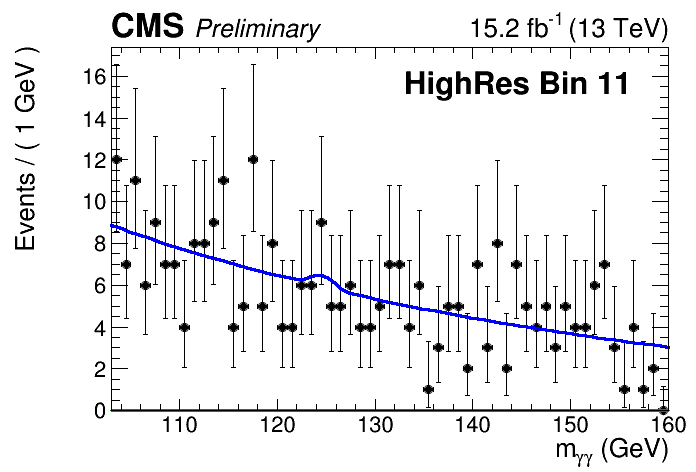
\includegraphics[width=0.45\textwidth, angle=0.]{figs/unblindedResults2p3Plus12p9/highResBin11_fit_b.png}
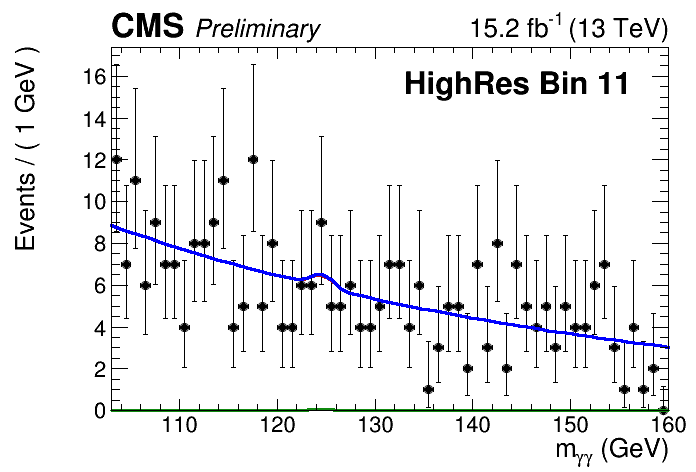
\includegraphics[width=0.45\textwidth, angle=0.]{figs/unblindedResults2p3Plus12p9/highResBin11_fit_s.png}\\
LowRes: $150 < M_{R} < 250$\GeV, $0 < R^{2}>0.175$\\
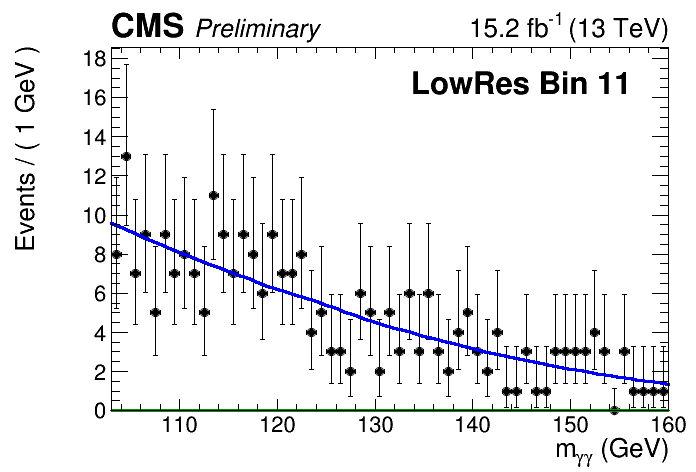
\includegraphics[width=0.45\textwidth, angle=0.]{figs/unblindedResults2p3Plus12p9/lowResBin11_fit_b.png}
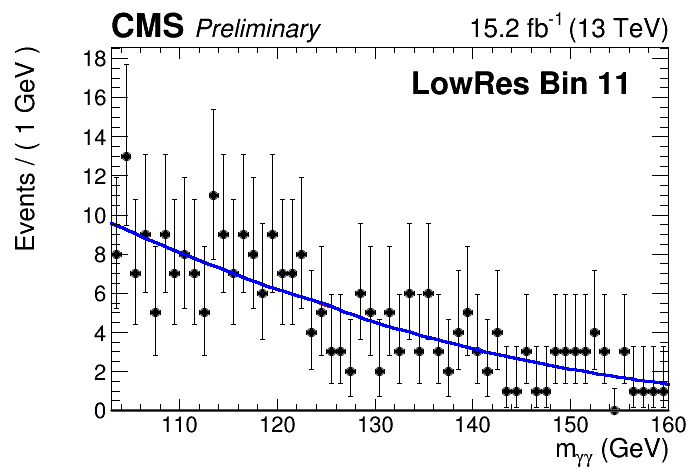
\includegraphics[width=0.45\textwidth, angle=0.]{figs/unblindedResults2p3Plus12p9/lowResBin11_fit_s.png}\\
\caption{ The diphoton mass distribution for the search region bin 11 
are shown along with the background-only fit (left) and the signal plus background fit (right).
The top row shows the HighRes category, while the bottom row shows the LowRes category.
The red curve represents the background prediction; the green curve represents the signal; 
and the blue curve represents the sum of the signal and background. The definition of the bin
is labeled above each pair of plots.
\label{fig:UnblindedResultsBin11}}
\end{figure}

\begin{figure}[ht!]
\centering
HighRes: $150 < M_{R} < 250$\GeV, $0 < R^{2}>0.175$\\
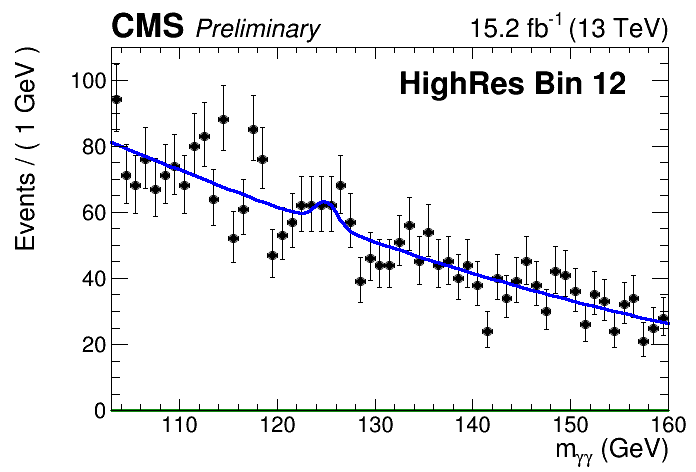
\includegraphics[width=0.45\textwidth, angle=0.]{figs/unblindedResults2p3Plus12p9/highResBin12_fit_b.png}
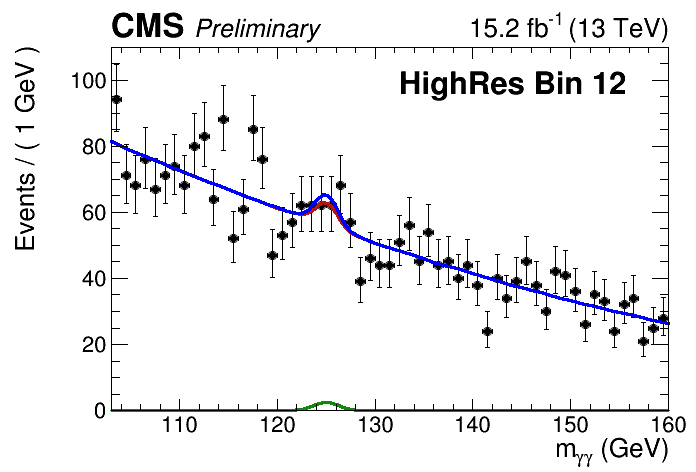
\includegraphics[width=0.45\textwidth, angle=0.]{figs/unblindedResults2p3Plus12p9/highResBin12_fit_s.png}\\
LowRes: $150 < M_{R} < 250$\GeV, $0 < R^{2}>0.175$\\
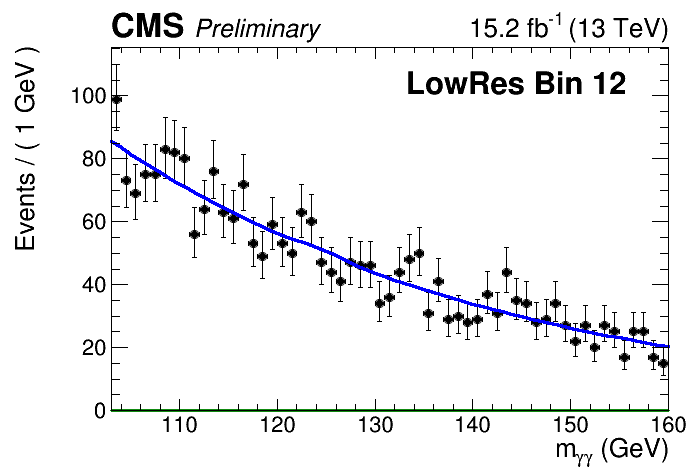
\includegraphics[width=0.45\textwidth, angle=0.]{figs/unblindedResults2p3Plus12p9/lowResBin12_fit_b.png}
\includegraphics[width=0.45\textwidth, angle=0.]{figs/unblindedResults2p3Plus12p9/lowResBin12_fit_s.png}\\
\caption{ The diphoton mass distribution for the search region bin 12 
are shown along with the background-only fit (left) and the signal plus background fit (right).
The top row shows the HighRes category, while the bottom row shows the LowRes category.
The red curve represents the background prediction; the green curve represents the signal; 
and the blue curve represents the sum of the signal and background. The definition of the bin
is labeled above each pair of plots.
\label{fig:UnblindedResultsBin12}}
\end{figure}

\begin{figure}[ht!]
\centering
HighRes: $150 < M_{R} < 250$\GeV, $0 < R^{2}>0.175$\\
\includegraphics[width=0.45\textwidth, angle=0.]{figs/unblindedResults2p3Plus12p9/highResBin13_fit_b.png}
\includegraphics[width=0.45\textwidth, angle=0.]{figs/unblindedResults2p3Plus12p9/highResBin13_fit_s.png}\\
LowRes: $150 < M_{R} < 250$\GeV, $0 < R^{2}>0.175$\\
\includegraphics[width=0.45\textwidth, angle=0.]{figs/unblindedResults2p3Plus12p9/lowResBin13_fit_b.png}
\includegraphics[width=0.45\textwidth, angle=0.]{figs/unblindedResults2p3Plus12p9/lowResBin13_fit_s.png}\\
\caption{ The diphoton mass distribution for the search region bin 13 
are shown along with the background-only fit (left) and the signal plus background fit (right).
The top row shows the HighRes category, while the bottom row shows the LowRes category.
The red curve represents the background prediction; the green curve represents the signal; 
and the blue curve represents the sum of the signal and background. The definition of the bin
is labeled above each pair of plots.
\label{fig:UnblindedResultsBin13}}
\end{figure}

The data yields, expected background yields, and best fit signal yields 
are summarized in Table~\ref{tab:bkgYieldTable} for all search region bins, together with the 
local statistical significance of the excess for each bin. The observed signal 
significance is summarized in Figure~\ref{fig:Significance} for all statistically independent bins.
The bin with the largest significance occurs in the HighPt category with $M_{R}>600$~GeV and $R^{2}>0.025$,
and has a local significance of $2.5\sigma$. Accounting for the number of search region bins,
this corresponds to a global significance of $1.4\sigma$.

\begin{table*}[h]
\begin{center}
\topcaption{The non-resonant background yields, 
SM Higgs background yields, best fit signal yields,
and observed local significance are shown for the signal plus background fit in 
each search region bin. The uncertainties include both statistical
and systematic components. The non-resonant background yields shown 
correspond to the yield within the window between $122$~GeV and $129$~GeV
and is intended to better reflect the background under the signal peak.
The observed significance for the bins in HighRes and LowRes categories are
identical because they are the result of a simultaneous fit. 
The significance is computed using the profile likelihood, where the sign
reflects whether an excess (positive sign) or deficit (negative sign) is observed. 
}
% Needs updated prefit Higgs bkg numbers from cristian's latest fits
\tiny
\begin{tabular}{|cc|cccc|c|}
\hline
           &          &                   & Yields        &                 &                        & Obs. Local     \\ 
Bin        & Category &  Non-Resonant Bkg & Exp. SM Higgs & Fitted SM Higgs &  Best Fit Signal       & Significance   \\ 
\hline
0          & HighPt   &  10.2 $\pm$ 1.4   & 2.0 $\pm$ 0.4    & 2.0 $\pm$ 0.7    & 9.7 $\pm$ 5.1      & $2.5 \sigma$     \\
1          & HighPt   &  10.5 $\pm$ 1.3   & 1.4 $\pm$ 0.3    & 1.4 $\pm$ 0.3    & 0.5 $\pm$ 3.4      & $0.2 \sigma$     \\
2          & HighPt   &  10.5 $\pm$ 1.6   & 3.0 $\pm$ 0.6    & 2.9 $\pm$ 0.9    & -5.2 $\pm$ 2.5     & $-1.4 \sigma$    \\
3          & HighPt   &  304 $\pm$ 16.6   & 27.7 $\pm$ 8.0  & 27.7 $\pm$ 11.2  & -7.9 $\pm$ 18.1    & $-0.4 \sigma$    \\
4          & HighPt   &  60 $\pm$ 3.0     & 8.8 $\pm$ 2.5    & 8.8 $\pm$ 3.5    & -13.9 $\pm$ 6.6    & $-1.6 \sigma$    \\
5          & HighPt   &  12.1 $\pm$ 1.4   & 1.7 $\pm$ 0.4    & 1.7 $\pm$ 0.6    & 8.3 $\pm$ 4.7      & $1.9 \sigma$     \\
6          & HighPt   &  47.6 $\pm$ 2.6   & 10.7 $\pm$ 2.7   & 10.7 $\pm$ 3.7   & 4.1 $\pm$ 7.3      & $0.6 \sigma$     \\
7          & HighPt   &  13.1 $\pm$ 1.4   & 2.7 $\pm$ 0.8    & 2.7 $\pm$ 1.0    & 3.2 $\pm$ 4.1      & $0.8 \sigma$     \\
\hline
8          & H($\gamma\gamma$)-H/Z(bb)     &  21.6 $\pm$ 1.8   & 1.0 $\pm$ 0.2    & 1.0 $\pm$ 0.2    & 5.3 $\pm$ 4.6      & $1.0 \sigma$    \\
\hline
9          & HighRes  &  697 $\pm$ 10.6   & 33.5 $\pm$ 10.4  & 33.2 $\pm$ 12.1  & 0.0 $\pm$ 21.4     &  $-0.2 \sigma$   \\ %should rerun with scale variation nuisance parameter combined
10         & HighRes  &  9.8 $\pm$ 1.2    & 0.6 $\pm$ 0.1    & 0.6 $\pm$ 0.1    & 8.2 $\pm$ 4.1      &  $1.7 \sigma$    \\ 
11         & HighRes  &  40.7 $\pm$ 2.4   & 1.7 $\pm$ 0.4    & 1.7 $\pm$ 0.6    & 0.2 $\pm$ 5.5      &  $0.0 \sigma$    \\ 
12         & HighRes  &  387 $\pm$ 14.6   & 21.5 $\pm$ 5.4   & 21.5 $\pm$ 9.1   & 8.1 $\pm$ 14.9     &  $0.5 \sigma$    \\ 
13         & HighRes  &  46.8 $\pm$ 2.6   & 3.5 $\pm$ 1.0    & 3.5 $\pm$ 1.2    & 1.3 $\pm$ 6.0      &  $0.2 \sigma$    \\ 
\hline                                                                          
9          & LowRes   &  591 $\pm$ 9      & 11.6 $\pm$ 3.8   & 11.9 $\pm$ 5.1   & 0.2 $\pm$ 10.1     & $-0.2 \sigma$    \\
10         & LowRes   &  14.1 $\pm$ 1.4   & 0.2 $\pm$ 0.1    & 0.2 $\pm$ 0.1    & 1.1 $\pm$ 0.8      & $1.7 \sigma$     \\
11         & LowRes   &  36.6 $\pm$ 9.2   & 0.6 $\pm$ 0.3    & 0.6 $\pm$ 0.3    & 0.1 $\pm$ 1.8      & $0.0 \sigma$     \\
12         & LowRes   &  341  $\pm$ 7     & 7.9 $\pm$ 2.3    & 7.9 $\pm$ 3.5    & 2.8 $\pm$ 5.0      & $0.5 \sigma$     \\
13         & LowRes   &  44.3 $\pm$ 2.4   & 1.4 $\pm$ 0.4    & 1.4 $\pm$ 0.7    & 0.5 $\pm$ 2.6      & $0.2 \sigma$     \\
\hline
\end{tabular}
\label{tab:bkgYieldTable}
\end{center}
\end{table*}




\begin{figure}[ht!]
\centering
\includegraphics[width=0.75\textwidth, angle=0.]{figs/SignificanceVsBin.pdf}
\caption{ 
The observed significance in units of standard deviations
is plotted for each search bin. The significance is computed using the profile likelihood, where the sign
reflects whether an excess (positive sign) or deficit (negative sign) is observed. 
The categories that the bins belong to are labeled at the bottom.
The yellow and green bands represent the $1\sigma$ and $2\sigma$
regions, respectively. 
\label{fig:Significance}}
\end{figure}


We interpret these results in terms of limits on the production cross-section times
branching ratio for sbottom pair production with a cascade decay to a Higgs 
boson, a bottom quark, and the LSP. The expected and observed limits on the sbottom pair production cross section 
is shown in Figure~\ref{fig:Limits} as a function of the
sbottom mass and the LSP mass. The observe significance is also
computed for this simplified model and shown in Figure~\ref{hgg:significance}.

\begin{figure}[ht!]
\centering
%\includegraphics[width=0.45\textwidth, angle=0.]{figs/limits/T2bHXSEC_OBSONLY.pdf}
%\includegraphics[width=0.45\textwidth,
%angle=0.]{figs/limits/T2bHXSEC_EXPONLY.pdf}
%\includegraphics[width=0.45\textwidth,angle=0.]{figs/limits/T2bH_Smooth_July31_XSEC.pdf}
\includegraphics[width=0.6\textwidth,angle=0.]{figs/limits/T2bH_Aug2XSEC.pdf}
\caption{ 
The observed 95\% confidence level (C.L.) upper limits on the production cross section
for sbottom pair production decaying to a bottom quark, a Higgs boson, and the LSP
are shown. The solid and dotted black contours represent the observed exclusion region and
its $1\sigma$ bands, while the analogous blue contours represent the expected
exclusion region and its $1\sigma$ bands.
\label{fig:Limits}}
\end{figure}
\begin{figure}[ht!]
\centering
%\includegraphics[width=0.45\textwidth, angle=0.]{figs/limits/T2bHXSEC_OBSONLY.pdf}
%\includegraphics[width=0.45\textwidth,
%angle=0.]{figs/limits/T2bHXSEC_EXPONLY.pdf}
%\includegraphics[width=0.45\textwidth,angle=0.]{figs/limits/T2bH_Smooth_July31_XSEC.pdf}
\includegraphics[width=0.6\textwidth,angle=0.]{hgg/T2bH_SignificanceXSEC.pdf}
\caption{ The observed significance scan for sbottom pair production
  decaying to a bottom quark, a Higgs boson, and the LSP is shown.
\label{hgg:significance}}
\end{figure}


\section{Summary}

A search for anomalous Higgs boson production through decays of supersymmetric particles is performed with
data collected in 2015 and 2016 by the CMS experiment at the CERN LHC. Proton collisions collected at a center-of-mass energy 
$\sqrt{s}=13$~TeV are considered, corresponding to an integrated luminosity of about 
15.2\fbinv (2.3\fbinv from 2015 and 12.9\fbinv from 2016). Higgs boson candidates are reconstructed from 
pairs of photons in the central part of the detector. The razor variables $M_{R}$ and $R^{2}$ are used to 
suppress SM Higgs boson production and other SM processes. The non-resonant background is estimated through a 
data-driven fit to the diphoton mass distribution using a functional form model selected
by a combination of the AIC score and the result of a series of bias tests. The standard model Higgs background
is estimated using the Monte Carlo simulation, with systematics on instrumental and theoretical uncertainties
propagated. We interpret the results in terms of production cross-section limits on sbottom pair production
each decaying to a Higgs boson, a b-quark, and the LSP, and exclude sbottoms with mass below $350$~GeV.

